\documentclass[twoside]{book}

% Packages required by doxygen
\usepackage{fixltx2e}
\usepackage{calc}
\usepackage{doxygen}
\usepackage{graphicx}
\usepackage[utf8]{inputenc}
\usepackage{makeidx}
\usepackage{multicol}
\usepackage{multirow}
\PassOptionsToPackage{warn}{textcomp}
\usepackage{textcomp}
\usepackage[nointegrals]{wasysym}
\usepackage[table]{xcolor}

% Font selection
\usepackage[T1]{fontenc}
\usepackage{mathptmx}
\usepackage[scaled=.90]{helvet}
\usepackage{courier}
\usepackage{amssymb}
\usepackage{sectsty}
\renewcommand{\familydefault}{\sfdefault}
\allsectionsfont{%
  \fontseries{bc}\selectfont%
  \color{darkgray}%
}
\renewcommand{\DoxyLabelFont}{%
  \fontseries{bc}\selectfont%
  \color{darkgray}%
}
\newcommand{\+}{\discretionary{\mbox{\scriptsize$\hookleftarrow$}}{}{}}

% Page & text layout
\usepackage{geometry}
\geometry{%
  a4paper,%
  top=2.5cm,%
  bottom=2.5cm,%
  left=2.5cm,%
  right=2.5cm%
}
\tolerance=750
\hfuzz=15pt
\hbadness=750
\setlength{\emergencystretch}{15pt}
\setlength{\parindent}{0cm}
\setlength{\parskip}{0.2cm}
\makeatletter
\renewcommand{\paragraph}{%
  \@startsection{paragraph}{4}{0ex}{-1.0ex}{1.0ex}{%
    \normalfont\normalsize\bfseries\SS@parafont%
  }%
}
\renewcommand{\subparagraph}{%
  \@startsection{subparagraph}{5}{0ex}{-1.0ex}{1.0ex}{%
    \normalfont\normalsize\bfseries\SS@subparafont%
  }%
}
\makeatother

% Headers & footers
\usepackage{fancyhdr}
\pagestyle{fancyplain}
\fancyhead[LE]{\fancyplain{}{\bfseries\thepage}}
\fancyhead[CE]{\fancyplain{}{}}
\fancyhead[RE]{\fancyplain{}{\bfseries\leftmark}}
\fancyhead[LO]{\fancyplain{}{\bfseries\rightmark}}
\fancyhead[CO]{\fancyplain{}{}}
\fancyhead[RO]{\fancyplain{}{\bfseries\thepage}}
\fancyfoot[LE]{\fancyplain{}{}}
\fancyfoot[CE]{\fancyplain{}{}}
\fancyfoot[RE]{\fancyplain{}{\bfseries\scriptsize Generated on Mon Aug 17 2015 10\+:50\+:54 for Kinfu\+L\+S Client Server by Doxygen }}
\fancyfoot[LO]{\fancyplain{}{\bfseries\scriptsize Generated on Mon Aug 17 2015 10\+:50\+:54 for Kinfu\+L\+S Client Server by Doxygen }}
\fancyfoot[CO]{\fancyplain{}{}}
\fancyfoot[RO]{\fancyplain{}{}}
\renewcommand{\footrulewidth}{0.4pt}
\renewcommand{\chaptermark}[1]{%
  \markboth{#1}{}%
}
\renewcommand{\sectionmark}[1]{%
  \markright{\thesection\ #1}%
}

% Indices & bibliography
\usepackage{natbib}
\usepackage[titles]{tocloft}
\setcounter{tocdepth}{3}
\setcounter{secnumdepth}{5}
\makeindex

% Hyperlinks (required, but should be loaded last)
\usepackage{ifpdf}
\ifpdf
  \usepackage[pdftex,pagebackref=true]{hyperref}
\else
  \usepackage[ps2pdf,pagebackref=true]{hyperref}
\fi
\hypersetup{%
  colorlinks=true,%
  linkcolor=blue,%
  citecolor=blue,%
  unicode%
}

% Custom commands
\newcommand{\clearemptydoublepage}{%
  \newpage{\pagestyle{empty}\cleardoublepage}%
}


%===== C O N T E N T S =====

\begin{document}

% Titlepage & ToC
\hypersetup{pageanchor=false,
             bookmarks=true,
             bookmarksnumbered=true,
             pdfencoding=unicode
            }
\pagenumbering{roman}
\begin{titlepage}
\vspace*{7cm}
\begin{center}%
{\Large Kinfu\+L\+S Client Server }\\
\vspace*{1cm}
{\large Generated by Doxygen 1.8.8}\\
\vspace*{0.5cm}
{\small Mon Aug 17 2015 10:50:54}\\
\end{center}
\end{titlepage}
\clearemptydoublepage
\tableofcontents
\clearemptydoublepage
\pagenumbering{arabic}
\hypersetup{pageanchor=true}

%--- Begin generated contents ---
\chapter{Module Index}
\section{Modules}
Here is a list of all modules\+:\begin{DoxyCompactList}
\item \contentsline{section}{Backend\+Server}{\pageref{group___backend_server}}{}
\item \contentsline{section}{Dimensional\+Data\+Source}{\pageref{group___dimensional_data_source}}{}
\end{DoxyCompactList}

\chapter{Hierarchical Index}
\section{Class Hierarchy}
This inheritance list is sorted roughly, but not completely, alphabetically\+:\begin{DoxyCompactList}
\item \contentsline{section}{Compression\+Strategy}{\pageref{class_compression_strategy}}{}
\begin{DoxyCompactList}
\item \contentsline{section}{J\+P\+E\+G\+Strategy}{\pageref{class_j_p_e_g_strategy}}{}
\item \contentsline{section}{P\+N\+G\+Strategy}{\pageref{class_p_n_g_strategy}}{}
\end{DoxyCompactList}
\item \contentsline{section}{Current\+Frame\+Cloud\+View}{\pageref{struct_current_frame_cloud_view}}{}
\item \contentsline{section}{D\+D\+S\+Client}{\pageref{class_d_d_s_client}}{}
\item Decompression\+Strategy\begin{DoxyCompactList}
\item \contentsline{section}{J\+P\+E\+G\+Decompression}{\pageref{class_j_p_e_g_decompression}}{}
\end{DoxyCompactList}
\item \contentsline{section}{Depth\+Client}{\pageref{class_depth_client}}{}
\item \contentsline{section}{Depth\+Server}{\pageref{class_depth_server}}{}
\item \contentsline{section}{Depth\+Source}{\pageref{class_depth_source}}{}
\begin{DoxyCompactList}
\item \contentsline{section}{Dummy\+Source}{\pageref{class_dummy_source}}{}
\item \contentsline{section}{Kinect\+V2\+Source}{\pageref{class_kinect_v2_source}}{}
\item \contentsline{section}{Open\+N\+I\+Source}{\pageref{class_open_n_i_source}}{}
\end{DoxyCompactList}
\item \contentsline{section}{Frame}{\pageref{struct_frame}}{}
\item \contentsline{section}{Image\+View}{\pageref{struct_image_view}}{}
\item \contentsline{section}{Kin\+Fu\+L\+S\+App}{\pageref{struct_kin_fu_l_s_app}}{}
\item \contentsline{section}{Kinfu\+Processor}{\pageref{class_kinfu_processor}}{}
\item \contentsline{section}{Limited\+Queue}{\pageref{class_limited_queue}}{}
\item \contentsline{section}{mem\+\_\+encode}{\pageref{structmem__encode}}{}
\item \contentsline{section}{my\+\_\+source\+\_\+mgr}{\pageref{structmy__source__mgr}}{}
\item \contentsline{section}{Scene\+Cloud\+View}{\pageref{struct_scene_cloud_view}}{}
\item Stop\+Watch\begin{DoxyCompactList}
\item \contentsline{section}{Sampled\+Scope\+Time}{\pageref{struct_sampled_scope_time}}{}
\end{DoxyCompactList}
\end{DoxyCompactList}

\chapter{Class Index}
\section{Class List}
Here are the classes, structs, unions and interfaces with brief descriptions\+:\begin{DoxyCompactList}
\item\contentsline{section}{\hyperlink{class_compression_strategy}{Compression\+Strategy} \\*Abstract class which defines the used compression stategy and the implementation to convert a depth image to a compressed image }{\pageref{class_compression_strategy}}{}
\item\contentsline{section}{\hyperlink{struct_current_frame_cloud_view}{Current\+Frame\+Cloud\+View} }{\pageref{struct_current_frame_cloud_view}}{}
\item\contentsline{section}{\hyperlink{class_d_d_s_client}{D\+D\+S\+Client} \\*Class that handles the sending of compressed images to a backend server }{\pageref{class_d_d_s_client}}{}
\item\contentsline{section}{\hyperlink{class_depth_client}{Depth\+Client} \\*Class which represents a client who connected to the Backend\+Server }{\pageref{class_depth_client}}{}
\item\contentsline{section}{\hyperlink{class_depth_server}{Depth\+Server} \\*Class that serves as a receiver of depth data. The depth data is to be decompressed by a specified Decompression\+Strategy, converted to a Pointcloud and then saved to disk to be processed later }{\pageref{class_depth_server}}{}
\item\contentsline{section}{\hyperlink{class_depth_source}{Depth\+Source} \\*Abstract class that serves as a source of depth data. The depth data is to be compressed by a specified \hyperlink{class_compression_strategy}{Compression\+Strategy} and then sent to the backend server using a \hyperlink{class_d_d_s_client}{D\+D\+S\+Client} }{\pageref{class_depth_source}}{}
\item\contentsline{section}{\hyperlink{class_dummy_source}{Dummy\+Source} \\*Class that extends the abstract class \hyperlink{class_depth_source}{Depth\+Source}. Acts as a dummysource of depthimages by sending compressed images that have previously been recorded by another depthsource and have been saved locally in a directory }{\pageref{class_dummy_source}}{}
\item\contentsline{section}{\hyperlink{struct_frame}{Frame} \\*Class that represents a compressed frame }{\pageref{struct_frame}}{}
\item\contentsline{section}{\hyperlink{struct_image_view}{Image\+View} }{\pageref{struct_image_view}}{}
\item\contentsline{section}{\hyperlink{class_j_p_e_g_decompression}{J\+P\+E\+G\+Decompression} \\*Class that extends the abstract class Decompression\+Strategy. Offers the functionality to decompress a 12-\/bit J\+P\+E\+G-\/image to a depth matrix }{\pageref{class_j_p_e_g_decompression}}{}
\item\contentsline{section}{\hyperlink{class_j_p_e_g_strategy}{J\+P\+E\+G\+Strategy} \\*Class that extends the abstract class \hyperlink{class_compression_strategy}{Compression\+Strategy}. Offers the functionality to compress a depth matrix to a 12-\/bit J\+P\+E\+G-\/image }{\pageref{class_j_p_e_g_strategy}}{}
\item\contentsline{section}{\hyperlink{class_kinect_v2_source}{Kinect\+V2\+Source} \\*Class that extends the abstract class \hyperlink{class_depth_source}{Depth\+Source}. Links a Kinect2-\/interface to a private callback method. This method compresses the received frame with a specific \hyperlink{class_compression_strategy}{Compression\+Strategy} and sends it to the backend server using a \hyperlink{class_d_d_s_client}{D\+D\+S\+Client} }{\pageref{class_kinect_v2_source}}{}
\item\contentsline{section}{\hyperlink{struct_kin_fu_l_s_app}{Kin\+Fu\+L\+S\+App} }{\pageref{struct_kin_fu_l_s_app}}{}
\item\contentsline{section}{\hyperlink{class_kinfu_processor}{Kinfu\+Processor} \\*Class that processes saved pointclouds and converts them into a world pointcloud }{\pageref{class_kinfu_processor}}{}
\item\contentsline{section}{\hyperlink{class_limited_queue}{Limited\+Queue} \\*Class that acts as a queue with a limited size for Frames }{\pageref{class_limited_queue}}{}
\item\contentsline{section}{\hyperlink{structmem__encode}{mem\+\_\+encode} }{\pageref{structmem__encode}}{}
\item\contentsline{section}{\hyperlink{structmy__source__mgr}{my\+\_\+source\+\_\+mgr} }{\pageref{structmy__source__mgr}}{}
\item\contentsline{section}{\hyperlink{class_open_n_i_source}{Open\+N\+I\+Source} \\*Class that extends the abstract class \hyperlink{class_depth_source}{Depth\+Source}. Links an Open\+N\+I Grabber-\/interface to a private callback method. This method compresses the received frame with a specific \hyperlink{class_compression_strategy}{Compression\+Strategy} and sends it to the backend server using a \hyperlink{class_d_d_s_client}{D\+D\+S\+Client} }{\pageref{class_open_n_i_source}}{}
\item\contentsline{section}{\hyperlink{class_p_n_g_strategy}{P\+N\+G\+Strategy} \\*Class that extends the abstract class \hyperlink{class_compression_strategy}{Compression\+Strategy}. Offers the functionality to compress a depth matrix to a 16-\/bit P\+N\+G-\/image. T\+O\+D\+O }{\pageref{class_p_n_g_strategy}}{}
\item\contentsline{section}{\hyperlink{struct_sampled_scope_time}{Sampled\+Scope\+Time} }{\pageref{struct_sampled_scope_time}}{}
\item\contentsline{section}{\hyperlink{struct_scene_cloud_view}{Scene\+Cloud\+View} }{\pageref{struct_scene_cloud_view}}{}
\end{DoxyCompactList}

\chapter{File Index}
\section{File List}
Here is a list of all documented files with brief descriptions\+:\begin{DoxyCompactList}
\item\contentsline{section}{\hyperlink{_compression_strategy_8h}{Compression\+Strategy.\+h} \\*Abstract Class which defines the compression strategy for the received frames }{\pageref{_compression_strategy_8h}}{}
\item\contentsline{section}{\hyperlink{_config_reader_8h}{Config\+Reader.\+h} \\*Utility Class which gives access to certain configuration constants }{\pageref{_config_reader_8h}}{}
\item\contentsline{section}{\hyperlink{_d_d_s_client_8h}{D\+D\+S\+Client.\+h} \\*Handles the sending of compressed images to a backend server }{\pageref{_d_d_s_client_8h}}{}
\item\contentsline{section}{\hyperlink{_depth_client_8h}{Depth\+Client.\+h} \\*Class which represents a client who connected to the Backend\+Server }{\pageref{_depth_client_8h}}{}
\item\contentsline{section}{\hyperlink{_depth_server_8h}{Depth\+Server.\+h} \\*Class which receives compressed frames through boost\+::asio }{\pageref{_depth_server_8h}}{}
\item\contentsline{section}{\hyperlink{_depth_source_8h}{Depth\+Source.\+h} \\*Abstract class which provides a stream of compressed depthimages }{\pageref{_depth_source_8h}}{}
\item\contentsline{section}{\hyperlink{_dummy_source_8h}{Dummy\+Source.\+h} \\*Class which implements the \hyperlink{class_depth_source}{Depth\+Source} abstract class. Acts as a dummy source as it sends the frames located in a directory to the backendserver through a \hyperlink{class_d_d_s_client}{D\+D\+S\+Client} }{\pageref{_dummy_source_8h}}{}
\item\contentsline{section}{\hyperlink{_j_p_e_g_decompression_8h}{J\+P\+E\+G\+Decompression.\+h} \\*Class which expands Decompression\+Strategy by defining the J\+P\+E\+G-\/decompression for the received images }{\pageref{_j_p_e_g_decompression_8h}}{}
\item\contentsline{section}{\hyperlink{_j_p_e_g_strategy_8h}{J\+P\+E\+G\+Strategy.\+h} \\*Class which expands \hyperlink{class_compression_strategy}{Compression\+Strategy} by defining the J\+P\+E\+G-\/compression for the received frames }{\pageref{_j_p_e_g_strategy_8h}}{}
\item\contentsline{section}{{\bfseries Kinect\+V2\+Source.\+h} }{\pageref{_kinect_v2_source_8h}}{}
\item\contentsline{section}{{\bfseries Kinfu\+Processor.\+h} }{\pageref{_kinfu_processor_8h}}{}
\item\contentsline{section}{\hyperlink{_open_n_i_source_8h}{Open\+N\+I\+Source.\+h} \\*Class of Dimensional\+Data\+Source which uses an Open\+N\+I-\/camera to receive frames and uses a \hyperlink{class_compression_strategy}{Compression\+Strategy} to compress them }{\pageref{_open_n_i_source_8h}}{}
\item\contentsline{section}{\hyperlink{_p_n_g_strategy_8h}{P\+N\+G\+Strategy.\+h} \\*Class of Dimensional\+Data\+Source which handles 16-\/bit P\+N\+G-\/compression of single depthframe }{\pageref{_p_n_g_strategy_8h}}{}
\end{DoxyCompactList}

\chapter{Module Documentation}
\hypertarget{group___backend_server}{\section{Backend\+Server}
\label{group___backend_server}\index{Backend\+Server@{Backend\+Server}}
}


Backend\+Server connects with multiple Dimensional Data Source Clients and receives their compressed frames through a T\+C\+P-\/connection. These frames then get decompressed using a Decompression\+Strategy and converted to Pointclouds.  


\subsection*{Files}
\begin{DoxyCompactItemize}
\item 
file \hyperlink{_depth_client_8h}{Depth\+Client.\+h}
\begin{DoxyCompactList}\small\item\em Class which represents a client who connected to the Backend\+Server. \end{DoxyCompactList}\item 
file \hyperlink{_depth_server_8h}{Depth\+Server.\+h}
\begin{DoxyCompactList}\small\item\em Class which receives compressed frames through boost\+::asio. \end{DoxyCompactList}\end{DoxyCompactItemize}


\subsection{Detailed Description}
Backend\+Server connects with multiple Dimensional Data Source Clients and receives their compressed frames through a T\+C\+P-\/connection. These frames then get decompressed using a Decompression\+Strategy and converted to Pointclouds. 

\begin{DoxyVersion}{Version}
1.\+0 
\end{DoxyVersion}

\hypertarget{group___dimensional_data_source}{\section{Dimensional\+Data\+Source}
\label{group___dimensional_data_source}\index{Dimensional\+Data\+Source@{Dimensional\+Data\+Source}}
}


Dimensional Data Source provides a consistent stream of compressed mages and sends them to a backend server through a single T\+C\+P-\/connection using the Boost-\/libraries.  


\subsection*{Files}
\begin{DoxyCompactItemize}
\item 
file \hyperlink{_compression_strategy_8h}{Compression\+Strategy.\+h}
\begin{DoxyCompactList}\small\item\em Abstract Class which defines the compression strategy for the received frames. \end{DoxyCompactList}\item 
file \hyperlink{_config_reader_8h}{Config\+Reader.\+h}
\begin{DoxyCompactList}\small\item\em Utility Class which gives access to certain configuration constants. \end{DoxyCompactList}\item 
file \hyperlink{_d_d_s_client_8h}{D\+D\+S\+Client.\+h}
\begin{DoxyCompactList}\small\item\em Handles the sending of compressed images to a backend server. \end{DoxyCompactList}\item 
file \hyperlink{_depth_source_8h}{Depth\+Source.\+h}
\begin{DoxyCompactList}\small\item\em Abstract class which provides a stream of compressed depthimages. \end{DoxyCompactList}\item 
file \hyperlink{_dummy_source_8h}{Dummy\+Source.\+h}
\begin{DoxyCompactList}\small\item\em Class which implements the \hyperlink{class_depth_source}{Depth\+Source} abstract class. Acts as a dummy source as it sends the frames located in a directory to the backendserver through a \hyperlink{class_d_d_s_client}{D\+D\+S\+Client}. \end{DoxyCompactList}\item 
file \hyperlink{_j_p_e_g_decompression_8h}{J\+P\+E\+G\+Decompression.\+h}
\begin{DoxyCompactList}\small\item\em Class which expands Decompression\+Strategy by defining the J\+P\+E\+G-\/decompression for the received images. \end{DoxyCompactList}\item 
file \hyperlink{_j_p_e_g_strategy_8h}{J\+P\+E\+G\+Strategy.\+h}
\begin{DoxyCompactList}\small\item\em Class which expands \hyperlink{class_compression_strategy}{Compression\+Strategy} by defining the J\+P\+E\+G-\/compression for the received frames. \end{DoxyCompactList}\item 
file \hyperlink{_open_n_i_source_8h}{Open\+N\+I\+Source.\+h}
\begin{DoxyCompactList}\small\item\em Class of Dimensional\+Data\+Source which uses an Open\+N\+I-\/camera to receive frames and uses a \hyperlink{class_compression_strategy}{Compression\+Strategy} to compress them. \end{DoxyCompactList}\item 
file \hyperlink{_p_n_g_strategy_8h}{P\+N\+G\+Strategy.\+h}
\begin{DoxyCompactList}\small\item\em Class of Dimensional\+Data\+Source which handles 16-\/bit P\+N\+G-\/compression of single depthframe. \end{DoxyCompactList}\end{DoxyCompactItemize}


\subsection{Detailed Description}
Dimensional Data Source provides a consistent stream of compressed mages and sends them to a backend server through a single T\+C\+P-\/connection using the Boost-\/libraries. 

\begin{DoxyVersion}{Version}
1.\+0 
\end{DoxyVersion}

\chapter{Class Documentation}
\hypertarget{class_compression_strategy}{\section{Compression\+Strategy Class Reference}
\label{class_compression_strategy}\index{Compression\+Strategy@{Compression\+Strategy}}
}


Abstract class which defines the used compression stategy and the implementation to convert a depth image to a compressed image.  




{\ttfamily \#include $<$Compression\+Strategy.\+h$>$}

Inheritance diagram for Compression\+Strategy\+:\begin{figure}[H]
\begin{center}
\leavevmode
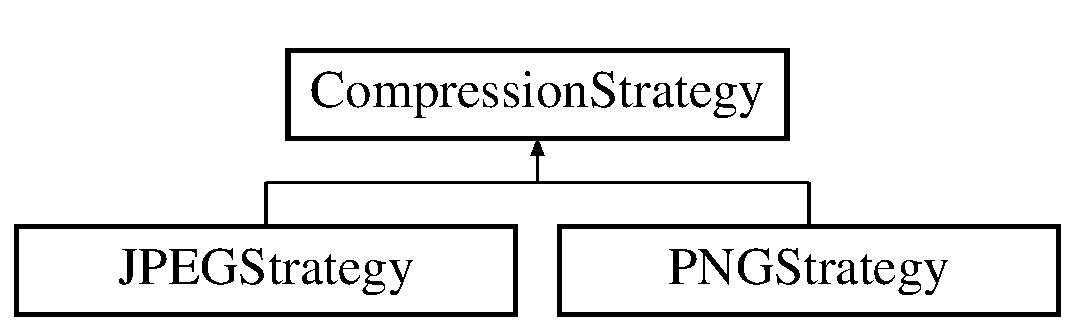
\includegraphics[height=2.000000cm]{class_compression_strategy}
\end{center}
\end{figure}
\subsection*{Public Member Functions}
\begin{DoxyCompactItemize}
\item 
virtual void \hyperlink{class_compression_strategy_a5124d2838fc7d8c769a34744f21602f4}{compress\+\_\+depth\+\_\+to\+\_\+image} (const int \&x\+Resolution, const int \&y\+Resolution, short $\ast$depth\+Data, unsigned char $\ast$\&out\+\_\+buffer\+\_\+, int \&n\+Bytes)=0
\begin{DoxyCompactList}\small\item\em Public method that offers the functionality to compress a depth matrix to a compressed image. \end{DoxyCompactList}\item 
\hypertarget{class_compression_strategy_af5a3cc25e0cad0b12544c6270f18dfb5}{virtual void {\bfseries decompress\+\_\+image\+\_\+to\+\_\+depth} (const int \&x\+Resolution, const int \&y\+Resolution, short $\ast$\&depth\+Data, unsigned char $\ast$image, int \&n\+Bytes)=0}\label{class_compression_strategy_af5a3cc25e0cad0b12544c6270f18dfb5}

\end{DoxyCompactItemize}


\subsection{Detailed Description}
Abstract class which defines the used compression stategy and the implementation to convert a depth image to a compressed image. 

\subsection{Member Function Documentation}
\hypertarget{class_compression_strategy_a5124d2838fc7d8c769a34744f21602f4}{\index{Compression\+Strategy@{Compression\+Strategy}!compress\+\_\+depth\+\_\+to\+\_\+image@{compress\+\_\+depth\+\_\+to\+\_\+image}}
\index{compress\+\_\+depth\+\_\+to\+\_\+image@{compress\+\_\+depth\+\_\+to\+\_\+image}!Compression\+Strategy@{Compression\+Strategy}}
\subsubsection[{compress\+\_\+depth\+\_\+to\+\_\+image}]{\setlength{\rightskip}{0pt plus 5cm}virtual void Compression\+Strategy\+::compress\+\_\+depth\+\_\+to\+\_\+image (
\begin{DoxyParamCaption}
\item[{const int \&}]{x\+Resolution, }
\item[{const int \&}]{y\+Resolution, }
\item[{short $\ast$}]{depth\+Data, }
\item[{unsigned char $\ast$\&}]{out\+\_\+buffer\+\_\+, }
\item[{int \&}]{n\+Bytes}
\end{DoxyParamCaption}
)\hspace{0.3cm}{\ttfamily [pure virtual]}}}\label{class_compression_strategy_a5124d2838fc7d8c769a34744f21602f4}


Public method that offers the functionality to compress a depth matrix to a compressed image. 


\begin{DoxyParams}[1]{Parameters}
\mbox{\tt in}  & {\em x\+Resolution} & The horizontal resolution of the used camera \\
\hline
\mbox{\tt in}  & {\em y\+Resolution} & The vertical resolution of the used camera \\
\hline
\mbox{\tt in}  & {\em depth\+Data} & A pointer to a depthmatrix containing the depth data \\
\hline
\mbox{\tt out}  & {\em out\+\_\+buffer} & A pointer to a databuffer containing the compressed image \\
\hline
\mbox{\tt out}  & {\em n\+Bytes} & The size of the out\+\_\+buffer in bytes \\
\hline
\end{DoxyParams}


Implemented in \hyperlink{class_p_n_g_strategy_aaa542a51c70ede4b82facb66d9ff9ec2}{P\+N\+G\+Strategy}, and \hyperlink{class_j_p_e_g_strategy_a3e27b992e48e592c4b127bbeeabc87ce}{J\+P\+E\+G\+Strategy}.



The documentation for this class was generated from the following file\+:\begin{DoxyCompactItemize}
\item 
\hyperlink{_compression_strategy_8h}{Compression\+Strategy.\+h}\end{DoxyCompactItemize}

\hypertarget{struct_current_frame_cloud_view}{\section{Current\+Frame\+Cloud\+View Struct Reference}
\label{struct_current_frame_cloud_view}\index{Current\+Frame\+Cloud\+View@{Current\+Frame\+Cloud\+View}}
}
\subsection*{Public Member Functions}
\begin{DoxyCompactItemize}
\item 
\hypertarget{struct_current_frame_cloud_view_a37675023be58802a2ed85a9d303cbc4c}{void {\bfseries show} (const Kinfu\+Tracker \&kinfu)}\label{struct_current_frame_cloud_view_a37675023be58802a2ed85a9d303cbc4c}

\item 
\hypertarget{struct_current_frame_cloud_view_ab11efdc7199b5ece6c97f751540ea112}{void {\bfseries set\+Viewer\+Pose} (const Eigen\+::\+Affine3f \&viewer\+\_\+pose)}\label{struct_current_frame_cloud_view_ab11efdc7199b5ece6c97f751540ea112}

\end{DoxyCompactItemize}
\subsection*{Public Attributes}
\begin{DoxyCompactItemize}
\item 
\hypertarget{struct_current_frame_cloud_view_a0757823c686e57a61b5bdb971cd4a08f}{Point\+Cloud$<$ Point\+X\+Y\+Z $>$\+::Ptr {\bfseries cloud\+\_\+ptr\+\_\+}}\label{struct_current_frame_cloud_view_a0757823c686e57a61b5bdb971cd4a08f}

\item 
\hypertarget{struct_current_frame_cloud_view_aa5752e2eaaab9b80dbd2b0b55b21a1df}{Device\+Array2\+D$<$ Point\+X\+Y\+Z $>$ {\bfseries cloud\+\_\+device\+\_\+}}\label{struct_current_frame_cloud_view_aa5752e2eaaab9b80dbd2b0b55b21a1df}

\item 
\hypertarget{struct_current_frame_cloud_view_a6458fec62b13b09a6b6caa78c864e698}{visualization\+::\+P\+C\+L\+Visualizer {\bfseries cloud\+\_\+viewer\+\_\+}}\label{struct_current_frame_cloud_view_a6458fec62b13b09a6b6caa78c864e698}

\end{DoxyCompactItemize}


The documentation for this struct was generated from the following file\+:\begin{DoxyCompactItemize}
\item 
kinfu\+L\+S\+\_\+app.\+cpp\end{DoxyCompactItemize}

\hypertarget{class_d_d_s_client}{\section{D\+D\+S\+Client Class Reference}
\label{class_d_d_s_client}\index{D\+D\+S\+Client@{D\+D\+S\+Client}}
}


Class that handles the sending of compressed images to a backend server.  




{\ttfamily \#include $<$D\+D\+S\+Client.\+h$>$}

\subsection*{Public Member Functions}
\begin{DoxyCompactItemize}
\item 
\hyperlink{class_d_d_s_client_a4d17bf120f9f3b3ec9e58010977f8de5}{D\+D\+S\+Client} (const int \&width\+\_\+, const int \&height\+\_\+, const \hyperlink{_compression_strategy_8h_a56a83bf6847f4801f4205eb4be237ccf}{Compression} \&comp\+\_\+)
\begin{DoxyCompactList}\small\item\em Constructor that establishes a connection with the backend server. \end{DoxyCompactList}\item 
\hypertarget{class_d_d_s_client_a3e3b8caddd8aa825f6895857591a4040}{\hyperlink{class_d_d_s_client_a3e3b8caddd8aa825f6895857591a4040}{$\sim$\+D\+D\+S\+Client} ()}\label{class_d_d_s_client_a3e3b8caddd8aa825f6895857591a4040}

\begin{DoxyCompactList}\small\item\em Destructor that closes the connection with the backend server if there's still a connection. \end{DoxyCompactList}\item 
\hypertarget{class_d_d_s_client_ab46ef5c251ae4896044436ed0443c17d}{void \hyperlink{class_d_d_s_client_ab46ef5c251ae4896044436ed0443c17d}{close\+Connection} ()}\label{class_d_d_s_client_ab46ef5c251ae4896044436ed0443c17d}

\begin{DoxyCompactList}\small\item\em Closes the connection with the backend server. \end{DoxyCompactList}\item 
bool \hyperlink{class_d_d_s_client_a93c7cf22bb7bd1fb663dd44406febecb}{send\+Frame\+To\+Server} (unsigned char $\ast$buf, const int \&size\+\_\+)
\begin{DoxyCompactList}\small\item\em Public method. Puts a single frame on the queue of frames remaining to send. \end{DoxyCompactList}\item 
\hypertarget{class_d_d_s_client_aaa2d92dfb333a3a2d3e2acb65c338e26}{void \hyperlink{class_d_d_s_client_aaa2d92dfb333a3a2d3e2acb65c338e26}{receive\+World\+From\+Server} ()}\label{class_d_d_s_client_aaa2d92dfb333a3a2d3e2acb65c338e26}

\begin{DoxyCompactList}\small\item\em Public method. Receives the size of the finished Kinfu\+World from the Backend Server, asynchronous. \end{DoxyCompactList}\item 
\hypertarget{class_d_d_s_client_a8c0e733323837567d33b0dbdc4472074}{string \hyperlink{class_d_d_s_client_a8c0e733323837567d33b0dbdc4472074}{get\+Host} ()}\label{class_d_d_s_client_a8c0e733323837567d33b0dbdc4472074}

\begin{DoxyCompactList}\small\item\em Public method. Gives a string which represents the I\+Pv4-\/address of the backendserver. \end{DoxyCompactList}\item 
\hypertarget{class_d_d_s_client_a21ad759ad351f9e77b22cec2c7353f57}{string \hyperlink{class_d_d_s_client_a21ad759ad351f9e77b22cec2c7353f57}{get\+Port} ()}\label{class_d_d_s_client_a21ad759ad351f9e77b22cec2c7353f57}

\begin{DoxyCompactList}\small\item\em Public method. Returns a string which represents the used port of the backendserver. \end{DoxyCompactList}\item 
\hypertarget{class_d_d_s_client_aeba51463ac23edc06f7384957d28f2f0}{void \hyperlink{class_d_d_s_client_aeba51463ac23edc06f7384957d28f2f0}{set\+Host} (const string \&host\+\_\+)}\label{class_d_d_s_client_aeba51463ac23edc06f7384957d28f2f0}

\begin{DoxyCompactList}\small\item\em Public method. Sets the I\+Pv4-\/address of the backend server. \end{DoxyCompactList}\item 
\hypertarget{class_d_d_s_client_a86b8c929d70c03ef84f84a32ae2e778e}{void \hyperlink{class_d_d_s_client_a86b8c929d70c03ef84f84a32ae2e778e}{set\+Port} (const string \&port\+\_\+)}\label{class_d_d_s_client_a86b8c929d70c03ef84f84a32ae2e778e}

\begin{DoxyCompactList}\small\item\em Public method. Sets the I\+Pv4-\/address of the backend server. \end{DoxyCompactList}\end{DoxyCompactItemize}


\subsection{Detailed Description}
Class that handles the sending of compressed images to a backend server. 

\subsection{Constructor \& Destructor Documentation}
\hypertarget{class_d_d_s_client_a4d17bf120f9f3b3ec9e58010977f8de5}{\index{D\+D\+S\+Client@{D\+D\+S\+Client}!D\+D\+S\+Client@{D\+D\+S\+Client}}
\index{D\+D\+S\+Client@{D\+D\+S\+Client}!D\+D\+S\+Client@{D\+D\+S\+Client}}
\subsubsection[{D\+D\+S\+Client}]{\setlength{\rightskip}{0pt plus 5cm}D\+D\+S\+Client\+::\+D\+D\+S\+Client (
\begin{DoxyParamCaption}
\item[{const int \&}]{width\+\_\+, }
\item[{const int \&}]{height\+\_\+, }
\item[{const {\bf Compression} \&}]{comp\+\_\+}
\end{DoxyParamCaption}
)\hspace{0.3cm}{\ttfamily [inline]}}}\label{class_d_d_s_client_a4d17bf120f9f3b3ec9e58010977f8de5}


Constructor that establishes a connection with the backend server. 


\begin{DoxyParams}[1]{Parameters}
\mbox{\tt in}  & {\em width\+\_\+} & The width of a single frame \\
\hline
\mbox{\tt in}  & {\em height\+\_\+} & The height of a single frame \\
\hline
\mbox{\tt in}  & {\em comp\+\_\+} & The used compression strategy \\
\hline
\end{DoxyParams}


\subsection{Member Function Documentation}
\hypertarget{class_d_d_s_client_a93c7cf22bb7bd1fb663dd44406febecb}{\index{D\+D\+S\+Client@{D\+D\+S\+Client}!send\+Frame\+To\+Server@{send\+Frame\+To\+Server}}
\index{send\+Frame\+To\+Server@{send\+Frame\+To\+Server}!D\+D\+S\+Client@{D\+D\+S\+Client}}
\subsubsection[{send\+Frame\+To\+Server}]{\setlength{\rightskip}{0pt plus 5cm}bool D\+D\+S\+Client\+::send\+Frame\+To\+Server (
\begin{DoxyParamCaption}
\item[{unsigned char $\ast$}]{buf, }
\item[{const int \&}]{size\+\_\+}
\end{DoxyParamCaption}
)\hspace{0.3cm}{\ttfamily [inline]}}}\label{class_d_d_s_client_a93c7cf22bb7bd1fb663dd44406febecb}


Public method. Puts a single frame on the queue of frames remaining to send. 


\begin{DoxyParams}[1]{Parameters}
\mbox{\tt in}  & {\em buf} & The buffer containing the compressed image \\
\hline
\mbox{\tt in}  & {\em size\+\_\+} & The size of the buffer (in bytes) \\
\hline
\end{DoxyParams}


The documentation for this class was generated from the following file\+:\begin{DoxyCompactItemize}
\item 
\hyperlink{_d_d_s_client_8h}{D\+D\+S\+Client.\+h}\end{DoxyCompactItemize}

\hypertarget{class_depth_client}{\section{Depth\+Client Class Reference}
\label{class_depth_client}\index{Depth\+Client@{Depth\+Client}}
}


Class which represents a client who connected to the Backend\+Server.  




{\ttfamily \#include $<$Depth\+Client.\+h$>$}

\subsection*{Public Member Functions}
\begin{DoxyCompactItemize}
\item 
\hyperlink{class_depth_client_a0e4751e122fcddf72547252a58ce46ab}{Depth\+Client} (boost\+::asio\+::io\+\_\+service \&io\+\_\+service, const int \&id\+\_\+, bool visualize\+Clouds\+\_\+=true)
\begin{DoxyCompactList}\small\item\em Public constructor which starts initializes the \hyperlink{class_depth_client}{Depth\+Client}. \end{DoxyCompactList}\item 
\hypertarget{class_depth_client_aa9682f7ce54fb6e87ae2fd6e1c668b7f}{tcp\+::socket \& \hyperlink{class_depth_client_aa9682f7ce54fb6e87ae2fd6e1c668b7f}{socket} ()}\label{class_depth_client_aa9682f7ce54fb6e87ae2fd6e1c668b7f}

\begin{DoxyCompactList}\small\item\em Public getter which returns the socket linked to the \hyperlink{class_depth_client}{Depth\+Client}. \end{DoxyCompactList}\item 
\hypertarget{class_depth_client_a32cc929b9902a4f9f488b1c609048cb5}{void \hyperlink{class_depth_client_a32cc929b9902a4f9f488b1c609048cb5}{start} ()}\label{class_depth_client_a32cc929b9902a4f9f488b1c609048cb5}

\begin{DoxyCompactList}\small\item\em Public method which starts the correspondance between the connected client and the server. \end{DoxyCompactList}\item 
\hypertarget{class_depth_client_ae13bf20205ccd9815a716ada83745794}{string {\bfseries get\+\_\+pointcloud\+\_\+path} (const int \&i)}\label{class_depth_client_ae13bf20205ccd9815a716ada83745794}

\item 
\hypertarget{class_depth_client_af6536183b766eded499d5fc2305838b6}{int {\bfseries get\+\_\+current\+\_\+frame} ()}\label{class_depth_client_af6536183b766eded499d5fc2305838b6}

\item 
\hypertarget{class_depth_client_a43c099aa7899efaf7f16ff0f1170b6c8}{bool {\bfseries is\+\_\+finished} ()}\label{class_depth_client_a43c099aa7899efaf7f16ff0f1170b6c8}

\item 
\hypertarget{class_depth_client_a7b7b8eff13e54fed9d40baccf4a2a506}{int {\bfseries get\+\_\+kinfu\+\_\+status} ()}\label{class_depth_client_a7b7b8eff13e54fed9d40baccf4a2a506}

\item 
\hypertarget{class_depth_client_a853118516fc4a72938448982f60e2613}{void {\bfseries set\+\_\+kinfu\+\_\+status} (int status)}\label{class_depth_client_a853118516fc4a72938448982f60e2613}

\end{DoxyCompactItemize}


\subsection{Detailed Description}
Class which represents a client who connected to the Backend\+Server. 

\subsection{Constructor \& Destructor Documentation}
\hypertarget{class_depth_client_a0e4751e122fcddf72547252a58ce46ab}{\index{Depth\+Client@{Depth\+Client}!Depth\+Client@{Depth\+Client}}
\index{Depth\+Client@{Depth\+Client}!Depth\+Client@{Depth\+Client}}
\subsubsection[{Depth\+Client}]{\setlength{\rightskip}{0pt plus 5cm}Depth\+Client\+::\+Depth\+Client (
\begin{DoxyParamCaption}
\item[{boost\+::asio\+::io\+\_\+service \&}]{io\+\_\+service, }
\item[{const int \&}]{id\+\_\+, }
\item[{bool}]{visualize\+Clouds\+\_\+ = {\ttfamily true}}
\end{DoxyParamCaption}
)\hspace{0.3cm}{\ttfamily [inline]}}}\label{class_depth_client_a0e4751e122fcddf72547252a58ce46ab}


Public constructor which starts initializes the \hyperlink{class_depth_client}{Depth\+Client}. 


\begin{DoxyParams}[1]{Parameters}
\mbox{\tt in}  & {\em io\+\_\+service} & The io\+\_\+service provided by boost\+::asio \\
\hline
\mbox{\tt in}  & {\em id\+\_\+} & The id of the \hyperlink{class_depth_client}{Depth\+Client} \\
\hline
\mbox{\tt in}  & {\em visualize\+Clouds} & Indicates if the received pointclouds should be visualized \\
\hline
\end{DoxyParams}


The documentation for this class was generated from the following file\+:\begin{DoxyCompactItemize}
\item 
\hyperlink{_depth_client_8h}{Depth\+Client.\+h}\end{DoxyCompactItemize}

\hypertarget{class_depth_server}{\section{Depth\+Server Class Reference}
\label{class_depth_server}\index{Depth\+Server@{Depth\+Server}}
}


Class that serves as a receiver of depth data. The depth data is to be decompressed by a specified Decompression\+Strategy, converted to a Pointcloud and then saved to disk to be processed later.  




{\ttfamily \#include $<$Depth\+Server.\+h$>$}

\subsection*{Public Member Functions}
\begin{DoxyCompactItemize}
\item 
\hyperlink{class_depth_server_a9ab59bd48e1280ee2dda1bdad4e6f8ff}{Depth\+Server} (boost\+::asio\+::io\+\_\+service \&io\+\_\+service, short port, bool visualize\+Clouds\+\_\+=false)
\begin{DoxyCompactList}\small\item\em Public constructor which starts the server on a given port and allows clients to connect. \end{DoxyCompactList}\item 
\hypertarget{class_depth_server_acf8fb886da8f5c4bd5b1c19e4267042a}{\hyperlink{class_depth_server_acf8fb886da8f5c4bd5b1c19e4267042a}{$\sim$\+Depth\+Server} ()}\label{class_depth_server_acf8fb886da8f5c4bd5b1c19e4267042a}

\begin{DoxyCompactList}\small\item\em Public destructor which starts the server on a given port and allows clients to connect. \end{DoxyCompactList}\item 
\hyperlink{class_depth_client}{Depth\+Client} $\ast$ \hyperlink{class_depth_server_a391a316cb888cee46324a137907c73f7}{get\+\_\+client} (const int \&i)
\begin{DoxyCompactList}\small\item\em Public getter which returns a pointer to a certain \hyperlink{class_depth_client}{Depth\+Client}. \end{DoxyCompactList}\item 
\hypertarget{class_depth_server_ad28c056c7576e2ff855e0d782d18b7e1}{int \hyperlink{class_depth_server_ad28c056c7576e2ff855e0d782d18b7e1}{get\+\_\+total\+\_\+clients} ()}\label{class_depth_server_ad28c056c7576e2ff855e0d782d18b7e1}

\begin{DoxyCompactList}\small\item\em Public getter which returns the total number of clients who have connected to the server. \end{DoxyCompactList}\item 
\hypertarget{class_depth_server_ae57fc68efb89381851e141be1dbe8ff2}{void \hyperlink{class_depth_server_ae57fc68efb89381851e141be1dbe8ff2}{handle\+\_\+accept} (\hyperlink{class_depth_client}{Depth\+Client} $\ast$new\+\_\+session, const boost\+::system\+::error\+\_\+code \&error)}\label{class_depth_server_ae57fc68efb89381851e141be1dbe8ff2}

\begin{DoxyCompactList}\small\item\em Public callbackmethod which handles a new \hyperlink{class_d_d_s_client}{D\+D\+S\+Client} connecting to the Backend\+Server. \end{DoxyCompactList}\end{DoxyCompactItemize}
\subsection*{Protected Attributes}
\begin{DoxyCompactItemize}
\item 
\hypertarget{class_depth_server_a8f00b5c9c633649786f2fc2929856b63}{boost\+::asio\+::io\+\_\+service \& {\bfseries io\+\_\+service\+\_\+}}\label{class_depth_server_a8f00b5c9c633649786f2fc2929856b63}

\item 
\hypertarget{class_depth_server_a80279520e474ba5bb2d9db12527bcc75}{tcp\+::acceptor {\bfseries acceptor\+\_\+}}\label{class_depth_server_a80279520e474ba5bb2d9db12527bcc75}

\item 
\hypertarget{class_depth_server_a2d934c3c2eaa2f9a4b55e2c659e42375}{vector$<$ \hyperlink{class_depth_client}{Depth\+Client} $\ast$ $>$ {\bfseries clients}}\label{class_depth_server_a2d934c3c2eaa2f9a4b55e2c659e42375}

\item 
\hypertarget{class_depth_server_adf38e34741b8085f85116cc806952c63}{int {\bfseries total\+\_\+clients}}\label{class_depth_server_adf38e34741b8085f85116cc806952c63}

\item 
\hypertarget{class_depth_server_a89a9934a17453d765d8872477afa70c0}{bool {\bfseries visualize\+Clouds}}\label{class_depth_server_a89a9934a17453d765d8872477afa70c0}

\end{DoxyCompactItemize}


\subsection{Detailed Description}
Class that serves as a receiver of depth data. The depth data is to be decompressed by a specified Decompression\+Strategy, converted to a Pointcloud and then saved to disk to be processed later. 

\subsection{Constructor \& Destructor Documentation}
\hypertarget{class_depth_server_a9ab59bd48e1280ee2dda1bdad4e6f8ff}{\index{Depth\+Server@{Depth\+Server}!Depth\+Server@{Depth\+Server}}
\index{Depth\+Server@{Depth\+Server}!Depth\+Server@{Depth\+Server}}
\subsubsection[{Depth\+Server}]{\setlength{\rightskip}{0pt plus 5cm}Depth\+Server\+::\+Depth\+Server (
\begin{DoxyParamCaption}
\item[{boost\+::asio\+::io\+\_\+service \&}]{io\+\_\+service, }
\item[{short}]{port, }
\item[{bool}]{visualize\+Clouds\+\_\+ = {\ttfamily false}}
\end{DoxyParamCaption}
)\hspace{0.3cm}{\ttfamily [inline]}}}\label{class_depth_server_a9ab59bd48e1280ee2dda1bdad4e6f8ff}


Public constructor which starts the server on a given port and allows clients to connect. 


\begin{DoxyParams}[1]{Parameters}
\mbox{\tt in}  & {\em io\+\_\+service} & The io\+\_\+service provided by boost \\
\hline
\mbox{\tt in}  & {\em port} & The port the server has to run on \\
\hline
\mbox{\tt in}  & {\em visualize\+Clouds\+\_\+} & Indicated if the received pointclouds should be visualized \\
\hline
\end{DoxyParams}


\subsection{Member Function Documentation}
\hypertarget{class_depth_server_a391a316cb888cee46324a137907c73f7}{\index{Depth\+Server@{Depth\+Server}!get\+\_\+client@{get\+\_\+client}}
\index{get\+\_\+client@{get\+\_\+client}!Depth\+Server@{Depth\+Server}}
\subsubsection[{get\+\_\+client}]{\setlength{\rightskip}{0pt plus 5cm}{\bf Depth\+Client}$\ast$ Depth\+Server\+::get\+\_\+client (
\begin{DoxyParamCaption}
\item[{const int \&}]{i}
\end{DoxyParamCaption}
)\hspace{0.3cm}{\ttfamily [inline]}}}\label{class_depth_server_a391a316cb888cee46324a137907c73f7}


Public getter which returns a pointer to a certain \hyperlink{class_depth_client}{Depth\+Client}. 


\begin{DoxyParams}[1]{Parameters}
\mbox{\tt in}  & {\em i} & The index of the \hyperlink{class_depth_client}{Depth\+Client} \\
\hline
\end{DoxyParams}


The documentation for this class was generated from the following file\+:\begin{DoxyCompactItemize}
\item 
\hyperlink{_depth_server_8h}{Depth\+Server.\+h}\end{DoxyCompactItemize}

\hypertarget{class_depth_source}{\section{Depth\+Source Class Reference}
\label{class_depth_source}\index{Depth\+Source@{Depth\+Source}}
}


Abstract class that serves as a source of depth data. The depth data is to be compressed by a specified \hyperlink{class_compression_strategy}{Compression\+Strategy} and then sent to the backend server using a \hyperlink{class_d_d_s_client}{D\+D\+S\+Client}.  




{\ttfamily \#include $<$Depth\+Source.\+h$>$}

Inheritance diagram for Depth\+Source\+:\begin{figure}[H]
\begin{center}
\leavevmode
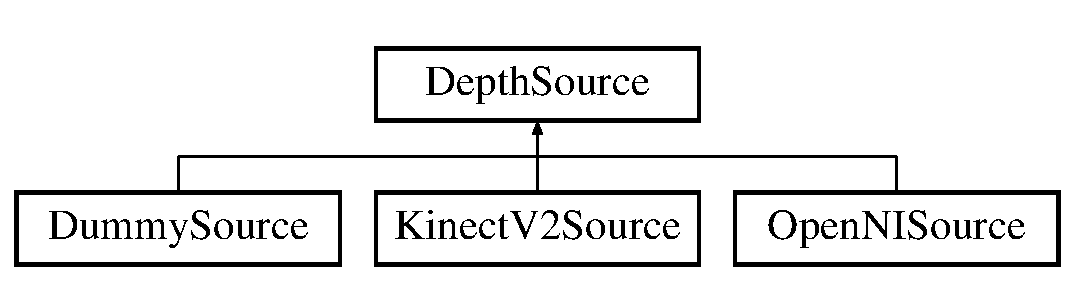
\includegraphics[height=2.000000cm]{class_depth_source}
\end{center}
\end{figure}
\subsection*{Public Member Functions}
\begin{DoxyCompactItemize}
\item 
\hypertarget{class_depth_source_a391f09ef6480e4243001381ab36c5d6b}{\hyperlink{class_depth_source_a391f09ef6480e4243001381ab36c5d6b}{Depth\+Source} (\hyperlink{_compression_strategy_8h_a56a83bf6847f4801f4205eb4be237ccf}{Compression} comp=J\+P\+E\+G)}\label{class_depth_source_a391f09ef6480e4243001381ab36c5d6b}

\begin{DoxyCompactList}\small\item\em Public constructor which initializes the correct \hyperlink{class_compression_strategy}{Compression\+Strategy}. \end{DoxyCompactList}\item 
\hypertarget{class_depth_source_a5d30215425a5816c488121bd9d770909}{virtual void \hyperlink{class_depth_source_a5d30215425a5816c488121bd9d770909}{run\+Depth\+Source} ()=0}\label{class_depth_source_a5d30215425a5816c488121bd9d770909}

\begin{DoxyCompactList}\small\item\em Public virtual method which starts the Grabber-\/interface. \end{DoxyCompactList}\item 
\hypertarget{class_depth_source_a524c199a0eabfec128d55dc676015f8d}{virtual void \hyperlink{class_depth_source_a524c199a0eabfec128d55dc676015f8d}{stop\+Depth\+Source} ()=0}\label{class_depth_source_a524c199a0eabfec128d55dc676015f8d}

\begin{DoxyCompactList}\small\item\em Public virtual method which stops the Grabber-\/interface. \end{DoxyCompactList}\item 
virtual void \hyperlink{class_depth_source_a9e15edc06570770976693b32ef7c5226}{save\+Frames\+To\+Directory} (const string \&directory\+\_\+, int N=M\+A\+X\+F\+I\+L\+E\+S)=0
\begin{DoxyCompactList}\small\item\em Virtual method.\+Saves a specified number of frames as to be determined images in a directory. \end{DoxyCompactList}\item 
\hypertarget{class_depth_source_ada5c09eba4cf325eea481e5acaefef76}{void {\bfseries set\+Server\+Settings} (const string \&address, const string \&port)}\label{class_depth_source_ada5c09eba4cf325eea481e5acaefef76}

\end{DoxyCompactItemize}
\subsection*{Protected Attributes}
\begin{DoxyCompactItemize}
\item 
\hypertarget{class_depth_source_aeda564a4cee4f9741fe44edb29982883}{\hyperlink{class_compression_strategy}{Compression\+Strategy} $\ast$ {\bfseries compression}}\label{class_depth_source_aeda564a4cee4f9741fe44edb29982883}

\item 
\hypertarget{class_depth_source_a24ca992b257e38717e9099f773eefd67}{\hyperlink{class_d_d_s_client}{D\+D\+S\+Client} $\ast$ {\bfseries client}}\label{class_depth_source_a24ca992b257e38717e9099f773eefd67}

\item 
\hypertarget{class_depth_source_a1ec315333dc0357859db36f281dcb568}{int {\bfseries frame}}\label{class_depth_source_a1ec315333dc0357859db36f281dcb568}

\item 
\hypertarget{class_depth_source_a7a1eb8572f2aa03d455f85a1b1709488}{int {\bfseries file\+Count}}\label{class_depth_source_a7a1eb8572f2aa03d455f85a1b1709488}

\item 
\hypertarget{class_depth_source_ac724a2f7d453e0ddad2e99bf3381f41f}{string {\bfseries D\+I\+R\+E\+C\+T\+O\+R\+Y}}\label{class_depth_source_ac724a2f7d453e0ddad2e99bf3381f41f}

\item 
\hypertarget{class_depth_source_a8682eac3aae4f214f9a33ff3ade2b1c7}{int {\bfseries x\+Resolution\+\_\+}}\label{class_depth_source_a8682eac3aae4f214f9a33ff3ade2b1c7}

\item 
\hypertarget{class_depth_source_a81392a74d51eb00a9b4abfa4a10938db}{int {\bfseries y\+Resolution\+\_\+}}\label{class_depth_source_a81392a74d51eb00a9b4abfa4a10938db}

\end{DoxyCompactItemize}
\subsection*{Static Protected Attributes}
\begin{DoxyCompactItemize}
\item 
\hypertarget{class_depth_source_a7da4336930cd7e2f5997bbb1b8bed5c7}{static const int {\bfseries M\+A\+X\+F\+I\+L\+E\+S} =5000}\label{class_depth_source_a7da4336930cd7e2f5997bbb1b8bed5c7}

\end{DoxyCompactItemize}


\subsection{Detailed Description}
Abstract class that serves as a source of depth data. The depth data is to be compressed by a specified \hyperlink{class_compression_strategy}{Compression\+Strategy} and then sent to the backend server using a \hyperlink{class_d_d_s_client}{D\+D\+S\+Client}. 

\subsection{Member Function Documentation}
\hypertarget{class_depth_source_a9e15edc06570770976693b32ef7c5226}{\index{Depth\+Source@{Depth\+Source}!save\+Frames\+To\+Directory@{save\+Frames\+To\+Directory}}
\index{save\+Frames\+To\+Directory@{save\+Frames\+To\+Directory}!Depth\+Source@{Depth\+Source}}
\subsubsection[{save\+Frames\+To\+Directory}]{\setlength{\rightskip}{0pt plus 5cm}virtual void Depth\+Source\+::save\+Frames\+To\+Directory (
\begin{DoxyParamCaption}
\item[{const string \&}]{directory\+\_\+, }
\item[{int}]{N = {\ttfamily MAXFILES}}
\end{DoxyParamCaption}
)\hspace{0.3cm}{\ttfamily [pure virtual]}}}\label{class_depth_source_a9e15edc06570770976693b32ef7c5226}


Virtual method.\+Saves a specified number of frames as to be determined images in a directory. 


\begin{DoxyParams}[1]{Parameters}
\mbox{\tt in}  & {\em directory} & The directory where the frames will be saved \\
\hline
\mbox{\tt in}  & {\em N} & The number of frames that have to be saved \\
\hline
\end{DoxyParams}


Implemented in \hyperlink{class_kinect_v2_source_a3fa31b0766bb3e9037bb72ef7e4baea7}{Kinect\+V2\+Source}, \hyperlink{class_dummy_source_af49cb371ea7e0eca894d1cdc26749f3f}{Dummy\+Source}, and \hyperlink{class_open_n_i_source_a2d6f642492a63ebb1cef48e927d52a06}{Open\+N\+I\+Source}.



The documentation for this class was generated from the following file\+:\begin{DoxyCompactItemize}
\item 
\hyperlink{_depth_source_8h}{Depth\+Source.\+h}\end{DoxyCompactItemize}

\hypertarget{class_dummy_source}{\section{Dummy\+Source Class Reference}
\label{class_dummy_source}\index{Dummy\+Source@{Dummy\+Source}}
}


Class that extends the abstract class \hyperlink{class_depth_source}{Depth\+Source}. Acts as a dummysource of depthimages by sending compressed images that have previously been recorded by another depthsource and have been saved locally in a directory.  




{\ttfamily \#include $<$Dummy\+Source.\+h$>$}

Inheritance diagram for Dummy\+Source\+:\begin{figure}[H]
\begin{center}
\leavevmode
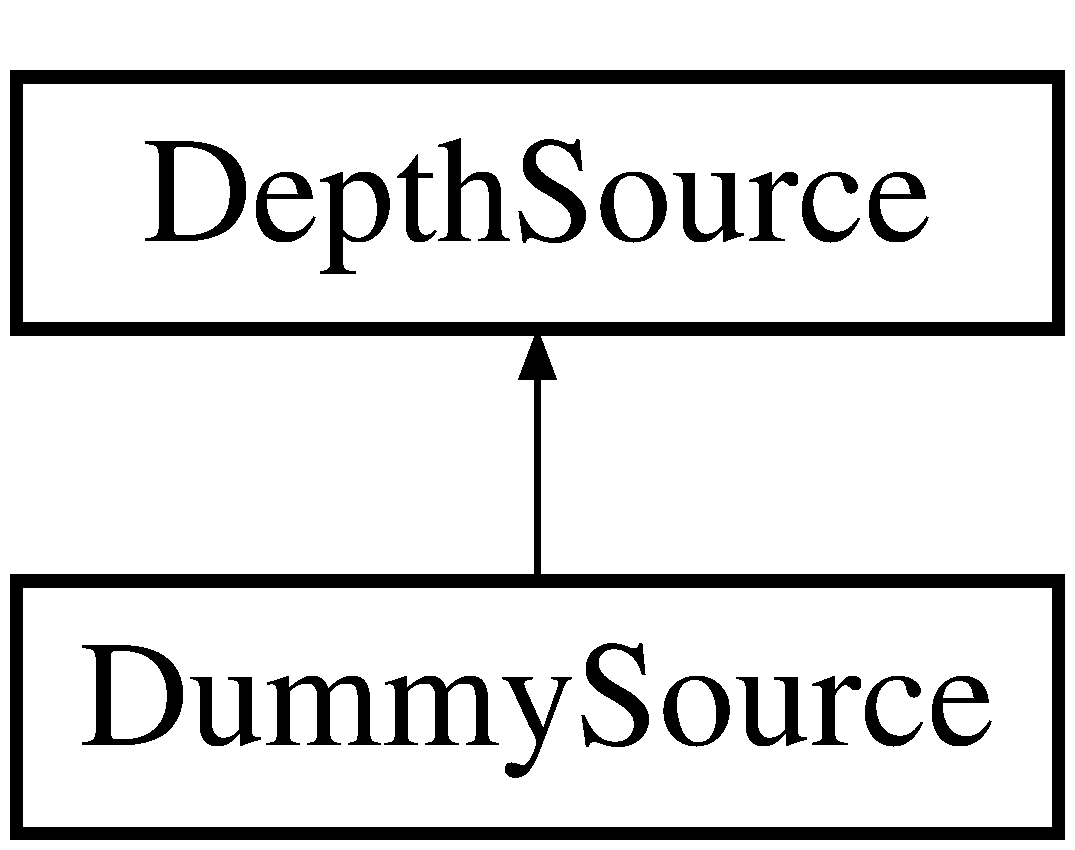
\includegraphics[height=2.000000cm]{class_dummy_source}
\end{center}
\end{figure}
\subsection*{Public Member Functions}
\begin{DoxyCompactItemize}
\item 
\hyperlink{class_dummy_source_a0909293c8d1f641619b0041e84adc06b}{Dummy\+Source} (const string \&directory, int x\+Resolution, int y\+Resolution, \hyperlink{_compression_strategy_8h_a56a83bf6847f4801f4205eb4be237ccf}{Compression} comp)
\begin{DoxyCompactList}\small\item\em Public constructor which initializes a connection with the \hyperlink{class_d_d_s_client}{D\+D\+S\+Client} and locates the directory needed. \end{DoxyCompactList}\item 
\hypertarget{class_dummy_source_a028993d5099e07fd5bde0b80dfd593bc}{\hyperlink{class_dummy_source_a028993d5099e07fd5bde0b80dfd593bc}{$\sim$\+Dummy\+Source} ()}\label{class_dummy_source_a028993d5099e07fd5bde0b80dfd593bc}

\begin{DoxyCompactList}\small\item\em Public destructor which terminates the connection with the backend server. \end{DoxyCompactList}\item 
\hypertarget{class_dummy_source_a93b6a46c6fc3b71488578b0bf1665bb6}{void \hyperlink{class_dummy_source_a93b6a46c6fc3b71488578b0bf1665bb6}{run\+Depth\+Source} ()}\label{class_dummy_source_a93b6a46c6fc3b71488578b0bf1665bb6}

\begin{DoxyCompactList}\small\item\em Public method which starts the dummysource and sends the frames located in the directory to the server. \end{DoxyCompactList}\item 
\hypertarget{class_dummy_source_a68186d8b68fac14eaaf764a50addbf14}{virtual void \hyperlink{class_dummy_source_a68186d8b68fac14eaaf764a50addbf14}{stop\+Depth\+Source} ()}\label{class_dummy_source_a68186d8b68fac14eaaf764a50addbf14}

\begin{DoxyCompactList}\small\item\em Public virtual method which stops the Grabber-\/interface. \end{DoxyCompactList}\item 
virtual void \hyperlink{class_dummy_source_af49cb371ea7e0eca894d1cdc26749f3f}{save\+Frames\+To\+Directory} (const string \&directory\+\_\+, int N=M\+A\+X\+F\+I\+L\+E\+S)
\begin{DoxyCompactList}\small\item\em Virtual method.\+Saves a specified number of frames as to be determined images in a directory. \end{DoxyCompactList}\end{DoxyCompactItemize}
\subsection*{Additional Inherited Members}


\subsection{Detailed Description}
Class that extends the abstract class \hyperlink{class_depth_source}{Depth\+Source}. Acts as a dummysource of depthimages by sending compressed images that have previously been recorded by another depthsource and have been saved locally in a directory. 

\subsection{Constructor \& Destructor Documentation}
\hypertarget{class_dummy_source_a0909293c8d1f641619b0041e84adc06b}{\index{Dummy\+Source@{Dummy\+Source}!Dummy\+Source@{Dummy\+Source}}
\index{Dummy\+Source@{Dummy\+Source}!Dummy\+Source@{Dummy\+Source}}
\subsubsection[{Dummy\+Source}]{\setlength{\rightskip}{0pt plus 5cm}Dummy\+Source\+::\+Dummy\+Source (
\begin{DoxyParamCaption}
\item[{const string \&}]{directory, }
\item[{int}]{x\+Resolution, }
\item[{int}]{y\+Resolution, }
\item[{{\bf Compression}}]{comp}
\end{DoxyParamCaption}
)\hspace{0.3cm}{\ttfamily [inline]}}}\label{class_dummy_source_a0909293c8d1f641619b0041e84adc06b}


Public constructor which initializes a connection with the \hyperlink{class_d_d_s_client}{D\+D\+S\+Client} and locates the directory needed. 


\begin{DoxyParams}[1]{Parameters}
\mbox{\tt in}  & {\em directory} & The directory where the frames are located \\
\hline
\mbox{\tt in}  & {\em x\+Resolution} & The horizontal resolution of the frames \\
\hline
\mbox{\tt in}  & {\em y\+Resolution} & The vertical resolution of the frames \\
\hline
\mbox{\tt in}  & {\em comp} & The used \hyperlink{class_compression_strategy}{Compression\+Strategy} \\
\hline
\end{DoxyParams}


\subsection{Member Function Documentation}
\hypertarget{class_dummy_source_af49cb371ea7e0eca894d1cdc26749f3f}{\index{Dummy\+Source@{Dummy\+Source}!save\+Frames\+To\+Directory@{save\+Frames\+To\+Directory}}
\index{save\+Frames\+To\+Directory@{save\+Frames\+To\+Directory}!Dummy\+Source@{Dummy\+Source}}
\subsubsection[{save\+Frames\+To\+Directory}]{\setlength{\rightskip}{0pt plus 5cm}virtual void Dummy\+Source\+::save\+Frames\+To\+Directory (
\begin{DoxyParamCaption}
\item[{const string \&}]{directory\+\_\+, }
\item[{int}]{N = {\ttfamily MAXFILES}}
\end{DoxyParamCaption}
)\hspace{0.3cm}{\ttfamily [inline]}, {\ttfamily [virtual]}}}\label{class_dummy_source_af49cb371ea7e0eca894d1cdc26749f3f}


Virtual method.\+Saves a specified number of frames as to be determined images in a directory. 


\begin{DoxyParams}[1]{Parameters}
\mbox{\tt in}  & {\em directory} & The directory where the frames will be saved \\
\hline
\mbox{\tt in}  & {\em N} & The number of frames that have to be saved \\
\hline
\end{DoxyParams}


Implements \hyperlink{class_depth_source_a9e15edc06570770976693b32ef7c5226}{Depth\+Source}.



The documentation for this class was generated from the following file\+:\begin{DoxyCompactItemize}
\item 
\hyperlink{_dummy_source_8h}{Dummy\+Source.\+h}\end{DoxyCompactItemize}

\hypertarget{struct_frame}{\section{Frame Struct Reference}
\label{struct_frame}\index{Frame@{Frame}}
}


Class that represents a compressed frame.  




{\ttfamily \#include $<$D\+D\+S\+Client.\+h$>$}

\subsection*{Public Member Functions}
\begin{DoxyCompactItemize}
\item 
\hypertarget{struct_frame_a1ed2cbc5161a5526db30b37c763bf7e6}{{\bfseries Frame} (unsigned char $\ast$\&buf\+\_\+, const int \&size\+\_\+)}\label{struct_frame_a1ed2cbc5161a5526db30b37c763bf7e6}

\end{DoxyCompactItemize}
\subsection*{Public Attributes}
\begin{DoxyCompactItemize}
\item 
\hypertarget{struct_frame_a5277685fd79d2a95cbfe4be6bd1d136b}{unsigned char $\ast$ {\bfseries buf}}\label{struct_frame_a5277685fd79d2a95cbfe4be6bd1d136b}

\item 
\hypertarget{struct_frame_a2c5a66a81df52f947008598cb2a0c281}{int {\bfseries size}}\label{struct_frame_a2c5a66a81df52f947008598cb2a0c281}

\end{DoxyCompactItemize}


\subsection{Detailed Description}
Class that represents a compressed frame. 

The documentation for this struct was generated from the following file\+:\begin{DoxyCompactItemize}
\item 
\hyperlink{_d_d_s_client_8h}{D\+D\+S\+Client.\+h}\end{DoxyCompactItemize}

\hypertarget{struct_image_view}{\section{Image\+View Struct Reference}
\label{struct_image_view}\index{Image\+View@{Image\+View}}
}
\subsection*{Public Member Functions}
\begin{DoxyCompactItemize}
\item 
\hypertarget{struct_image_view_af942dc3f5e83018d15c7b3033318e188}{void {\bfseries show\+Scene} (Kinfu\+Tracker \&kinfu, const Ptr\+Step\+Sz$<$ const pcl\+::gpu\+::kinfu\+L\+S\+::\+Pixel\+R\+G\+B $>$ \&rgb24, bool registration, Eigen\+::\+Affine3f $\ast$pose\+\_\+ptr=0)}\label{struct_image_view_af942dc3f5e83018d15c7b3033318e188}

\item 
\hypertarget{struct_image_view_a3bec20cc86e59d0c5bf2ad10913d9710}{void {\bfseries show\+Depth} (const Ptr\+Step\+Sz$<$ const unsigned short $>$ \&depth)}\label{struct_image_view_a3bec20cc86e59d0c5bf2ad10913d9710}

\item 
\hypertarget{struct_image_view_a791a70341165462534172328eb3057a9}{void {\bfseries show\+Generated\+Depth} (Kinfu\+Tracker \&kinfu, const Eigen\+::\+Affine3f \&pose)}\label{struct_image_view_a791a70341165462534172328eb3057a9}

\item 
\hypertarget{struct_image_view_a33190e1bb9e52398e2b7f5fc3ee16d48}{void {\bfseries toggle\+Image\+Paint} ()}\label{struct_image_view_a33190e1bb9e52398e2b7f5fc3ee16d48}

\end{DoxyCompactItemize}
\subsection*{Public Attributes}
\begin{DoxyCompactItemize}
\item 
\hypertarget{struct_image_view_a3d4f9ee3d67ace1efcbdb33b34e4b7e8}{bool {\bfseries paint\+\_\+image\+\_\+}}\label{struct_image_view_a3d4f9ee3d67ace1efcbdb33b34e4b7e8}

\item 
\hypertarget{struct_image_view_a381f921f4232aac9e8d5d51580cb4100}{bool {\bfseries accumulate\+\_\+views\+\_\+}}\label{struct_image_view_a381f921f4232aac9e8d5d51580cb4100}

\item 
\hypertarget{struct_image_view_a6f1ddcd6ff914ada3a21dd2735cd5c01}{visualization\+::\+Image\+Viewer {\bfseries viewer\+Scene\+\_\+}}\label{struct_image_view_a6f1ddcd6ff914ada3a21dd2735cd5c01}

\item 
\hypertarget{struct_image_view_a4f96bf1c879677d7e4389e304b9a4783}{visualization\+::\+Image\+Viewer {\bfseries viewer\+Depth\+\_\+}}\label{struct_image_view_a4f96bf1c879677d7e4389e304b9a4783}

\item 
\hypertarget{struct_image_view_a4357cf1bfa868a7a057cab2f464c3935}{Kinfu\+Tracker\+::\+View {\bfseries view\+\_\+device\+\_\+}}\label{struct_image_view_a4357cf1bfa868a7a057cab2f464c3935}

\item 
\hypertarget{struct_image_view_a97efc213c640548a3a80807482c6f79d}{Kinfu\+Tracker\+::\+View {\bfseries colors\+\_\+device\+\_\+}}\label{struct_image_view_a97efc213c640548a3a80807482c6f79d}

\item 
\hypertarget{struct_image_view_abff4f8ee5f883f26a9fd50a8fa7edcc8}{vector\\*
$<$ pcl\+::gpu\+::kinfu\+L\+S\+::\+Pixel\+R\+G\+B $>$ {\bfseries view\+\_\+host\+\_\+}}\label{struct_image_view_abff4f8ee5f883f26a9fd50a8fa7edcc8}

\item 
\hypertarget{struct_image_view_acc7f92b88be07d02a22330a6b70a3cf0}{Ray\+Caster\+::\+Ptr {\bfseries raycaster\+\_\+ptr\+\_\+}}\label{struct_image_view_acc7f92b88be07d02a22330a6b70a3cf0}

\item 
\hypertarget{struct_image_view_a7862bb641af08e7e4280c49b4fda87a6}{Kinfu\+Tracker\+::\+Depth\+Map {\bfseries generated\+\_\+depth\+\_\+}}\label{struct_image_view_a7862bb641af08e7e4280c49b4fda87a6}

\end{DoxyCompactItemize}


The documentation for this struct was generated from the following file\+:\begin{DoxyCompactItemize}
\item 
kinfu\+L\+S\+\_\+app.\+cpp\end{DoxyCompactItemize}

\hypertarget{class_j_p_e_g_decompression}{\section{J\+P\+E\+G\+Decompression Class Reference}
\label{class_j_p_e_g_decompression}\index{J\+P\+E\+G\+Decompression@{J\+P\+E\+G\+Decompression}}
}


Class that extends the abstract class Decompression\+Strategy. Offers the functionality to decompress a 12-\/bit J\+P\+E\+G-\/image to a depth matrix.  




{\ttfamily \#include $<$J\+P\+E\+G\+Decompression.\+h$>$}

Inheritance diagram for J\+P\+E\+G\+Decompression\+:\begin{figure}[H]
\begin{center}
\leavevmode
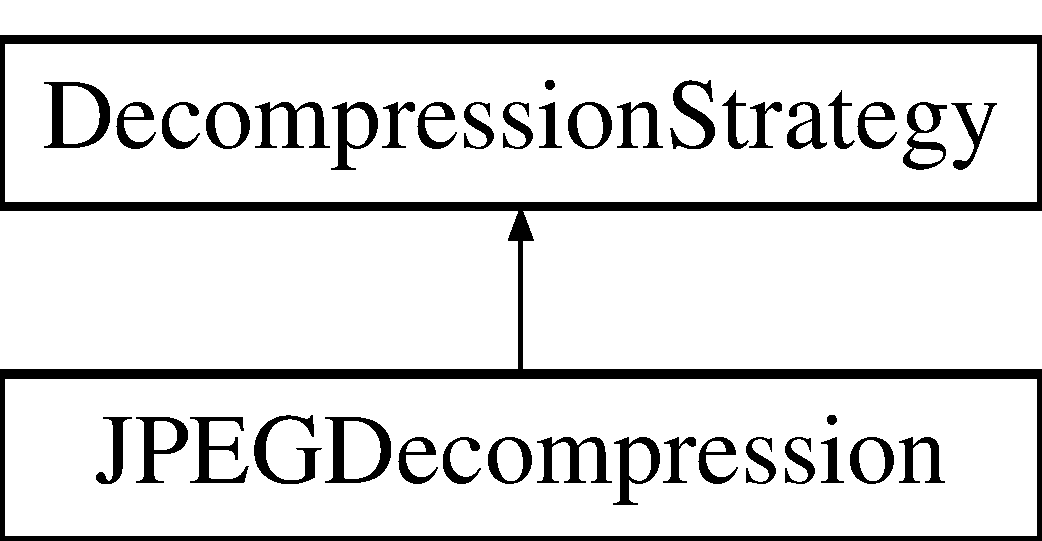
\includegraphics[height=2.000000cm]{class_j_p_e_g_decompression}
\end{center}
\end{figure}
\subsection*{Public Member Functions}
\begin{DoxyCompactItemize}
\item 
void \hyperlink{class_j_p_e_g_decompression_ad9f3e806d9e86a5333f37929c385496c}{decompress\+\_\+image\+\_\+to\+\_\+depth} (const int \&x\+Resolution, const int \&y\+Resolution, short $\ast$\&data, unsigned char $\ast$image)
\begin{DoxyCompactList}\small\item\em Public method that offers the functionality to compress a depth matrix to a 12-\/bit J\+P\+E\+G-\/image. \end{DoxyCompactList}\end{DoxyCompactItemize}


\subsection{Detailed Description}
Class that extends the abstract class Decompression\+Strategy. Offers the functionality to decompress a 12-\/bit J\+P\+E\+G-\/image to a depth matrix. 

\subsection{Member Function Documentation}
\hypertarget{class_j_p_e_g_decompression_ad9f3e806d9e86a5333f37929c385496c}{\index{J\+P\+E\+G\+Decompression@{J\+P\+E\+G\+Decompression}!decompress\+\_\+image\+\_\+to\+\_\+depth@{decompress\+\_\+image\+\_\+to\+\_\+depth}}
\index{decompress\+\_\+image\+\_\+to\+\_\+depth@{decompress\+\_\+image\+\_\+to\+\_\+depth}!J\+P\+E\+G\+Decompression@{J\+P\+E\+G\+Decompression}}
\subsubsection[{decompress\+\_\+image\+\_\+to\+\_\+depth}]{\setlength{\rightskip}{0pt plus 5cm}void J\+P\+E\+G\+Decompression\+::decompress\+\_\+image\+\_\+to\+\_\+depth (
\begin{DoxyParamCaption}
\item[{const int \&}]{x\+Resolution, }
\item[{const int \&}]{y\+Resolution, }
\item[{short $\ast$\&}]{data, }
\item[{unsigned char $\ast$}]{image}
\end{DoxyParamCaption}
)\hspace{0.3cm}{\ttfamily [inline]}}}\label{class_j_p_e_g_decompression_ad9f3e806d9e86a5333f37929c385496c}


Public method that offers the functionality to compress a depth matrix to a 12-\/bit J\+P\+E\+G-\/image. 


\begin{DoxyParams}[1]{Parameters}
\mbox{\tt in}  & {\em x\+Resolution} & The horizontal resolution of the used camera \\
\hline
\mbox{\tt in}  & {\em y\+Resolution} & The vertical resolution of the used camera \\
\hline
\mbox{\tt in}  & {\em depth\+Data} & A pointer to a depthmatrix containing the depth data \\
\hline
\mbox{\tt out}  & {\em out\+\_\+buffer} & A pointer to a databuffer containing the compressed image \\
\hline
\mbox{\tt out}  & {\em n\+Bytes} & The size of the out\+\_\+buffer in bytes \\
\hline
\end{DoxyParams}


The documentation for this class was generated from the following file\+:\begin{DoxyCompactItemize}
\item 
\hyperlink{_j_p_e_g_decompression_8h}{J\+P\+E\+G\+Decompression.\+h}\end{DoxyCompactItemize}

\hypertarget{class_j_p_e_g_strategy}{\section{J\+P\+E\+G\+Strategy Class Reference}
\label{class_j_p_e_g_strategy}\index{J\+P\+E\+G\+Strategy@{J\+P\+E\+G\+Strategy}}
}


Class that extends the abstract class \hyperlink{class_compression_strategy}{Compression\+Strategy}. Offers the functionality to compress a depth matrix to a 12-\/bit J\+P\+E\+G-\/image.  




{\ttfamily \#include $<$J\+P\+E\+G\+Strategy.\+h$>$}

Inheritance diagram for J\+P\+E\+G\+Strategy\+:\begin{figure}[H]
\begin{center}
\leavevmode
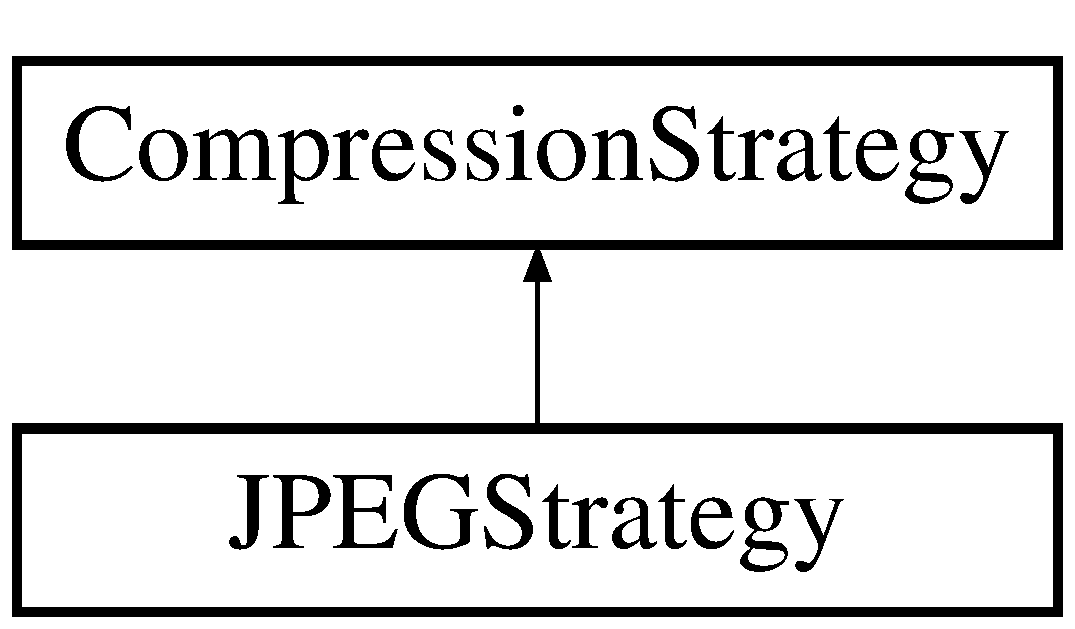
\includegraphics[height=2.000000cm]{class_j_p_e_g_strategy}
\end{center}
\end{figure}
\subsection*{Public Member Functions}
\begin{DoxyCompactItemize}
\item 
void \hyperlink{class_j_p_e_g_strategy_a3e27b992e48e592c4b127bbeeabc87ce}{compress\+\_\+depth\+\_\+to\+\_\+image} (const int \&x\+Resolution, const int \&y\+Resolution, short $\ast$depth\+Data, unsigned char $\ast$\&out\+\_\+buffer\+\_\+, int \&n\+Bytes)
\begin{DoxyCompactList}\small\item\em Public method that offers the functionality to compress a depth matrix to a 12-\/bit J\+P\+E\+G-\/image. \end{DoxyCompactList}\item 
void \hyperlink{class_j_p_e_g_strategy_ae1005fca6a7f6ac3a1ec7e603d0af01a}{decompress\+\_\+image\+\_\+to\+\_\+depth} (const int \&x\+Resolution, const int \&y\+Resolution, short $\ast$\&data, unsigned char $\ast$image, int \&n\+Bytes)
\begin{DoxyCompactList}\small\item\em Public method that offers the functionality to decompress a 12-\/bit J\+P\+E\+G-\/image to a depth matrix. \end{DoxyCompactList}\end{DoxyCompactItemize}


\subsection{Detailed Description}
Class that extends the abstract class \hyperlink{class_compression_strategy}{Compression\+Strategy}. Offers the functionality to compress a depth matrix to a 12-\/bit J\+P\+E\+G-\/image. 

\subsection{Member Function Documentation}
\hypertarget{class_j_p_e_g_strategy_a3e27b992e48e592c4b127bbeeabc87ce}{\index{J\+P\+E\+G\+Strategy@{J\+P\+E\+G\+Strategy}!compress\+\_\+depth\+\_\+to\+\_\+image@{compress\+\_\+depth\+\_\+to\+\_\+image}}
\index{compress\+\_\+depth\+\_\+to\+\_\+image@{compress\+\_\+depth\+\_\+to\+\_\+image}!J\+P\+E\+G\+Strategy@{J\+P\+E\+G\+Strategy}}
\subsubsection[{compress\+\_\+depth\+\_\+to\+\_\+image}]{\setlength{\rightskip}{0pt plus 5cm}void J\+P\+E\+G\+Strategy\+::compress\+\_\+depth\+\_\+to\+\_\+image (
\begin{DoxyParamCaption}
\item[{const int \&}]{x\+Resolution, }
\item[{const int \&}]{y\+Resolution, }
\item[{short $\ast$}]{depth\+Data, }
\item[{unsigned char $\ast$\&}]{out\+\_\+buffer\+\_\+, }
\item[{int \&}]{n\+Bytes}
\end{DoxyParamCaption}
)\hspace{0.3cm}{\ttfamily [inline]}, {\ttfamily [virtual]}}}\label{class_j_p_e_g_strategy_a3e27b992e48e592c4b127bbeeabc87ce}


Public method that offers the functionality to compress a depth matrix to a 12-\/bit J\+P\+E\+G-\/image. 


\begin{DoxyParams}[1]{Parameters}
\mbox{\tt in}  & {\em x\+Resolution} & The horizontal resolution of the used camera \\
\hline
\mbox{\tt in}  & {\em y\+Resolution} & The vertical resolution of the used camera \\
\hline
\mbox{\tt in}  & {\em depth\+Data} & A pointer to a depthmatrix containing the depth data \\
\hline
\mbox{\tt out}  & {\em out\+\_\+buffer} & A pointer to a databuffer containing the compressed image \\
\hline
\mbox{\tt out}  & {\em n\+Bytes} & The size of the out\+\_\+buffer in bytes \\
\hline
\end{DoxyParams}


Implements \hyperlink{class_compression_strategy_a5124d2838fc7d8c769a34744f21602f4}{Compression\+Strategy}.

\hypertarget{class_j_p_e_g_strategy_ae1005fca6a7f6ac3a1ec7e603d0af01a}{\index{J\+P\+E\+G\+Strategy@{J\+P\+E\+G\+Strategy}!decompress\+\_\+image\+\_\+to\+\_\+depth@{decompress\+\_\+image\+\_\+to\+\_\+depth}}
\index{decompress\+\_\+image\+\_\+to\+\_\+depth@{decompress\+\_\+image\+\_\+to\+\_\+depth}!J\+P\+E\+G\+Strategy@{J\+P\+E\+G\+Strategy}}
\subsubsection[{decompress\+\_\+image\+\_\+to\+\_\+depth}]{\setlength{\rightskip}{0pt plus 5cm}void J\+P\+E\+G\+Strategy\+::decompress\+\_\+image\+\_\+to\+\_\+depth (
\begin{DoxyParamCaption}
\item[{const int \&}]{x\+Resolution, }
\item[{const int \&}]{y\+Resolution, }
\item[{short $\ast$\&}]{data, }
\item[{unsigned char $\ast$}]{image, }
\item[{int \&}]{n\+Bytes}
\end{DoxyParamCaption}
)\hspace{0.3cm}{\ttfamily [inline]}, {\ttfamily [virtual]}}}\label{class_j_p_e_g_strategy_ae1005fca6a7f6ac3a1ec7e603d0af01a}


Public method that offers the functionality to decompress a 12-\/bit J\+P\+E\+G-\/image to a depth matrix. 


\begin{DoxyParams}[1]{Parameters}
\mbox{\tt in}  & {\em x\+Resolution} & The horizontal resolution of the used camera \\
\hline
\mbox{\tt in}  & {\em y\+Resolution} & The vertical resolution of the used camera \\
\hline
\mbox{\tt in}  & {\em depth\+Data} & A pointer to a depthmatrix containing the depth data \\
\hline
\mbox{\tt out}  & {\em out\+\_\+buffer} & A pointer to a databuffer containing the compressed image \\
\hline
\mbox{\tt out}  & {\em n\+Bytes} & The size of the out\+\_\+buffer in bytes \\
\hline
\end{DoxyParams}


Implements \hyperlink{class_compression_strategy}{Compression\+Strategy}.



The documentation for this class was generated from the following file\+:\begin{DoxyCompactItemize}
\item 
\hyperlink{_j_p_e_g_strategy_8h}{J\+P\+E\+G\+Strategy.\+h}\end{DoxyCompactItemize}

\hypertarget{class_kinect_v2_source}{\section{Kinect\+V2\+Source Class Reference}
\label{class_kinect_v2_source}\index{Kinect\+V2\+Source@{Kinect\+V2\+Source}}
}


Class that extends the abstract class \hyperlink{class_depth_source}{Depth\+Source}. Links a Kinect2-\/interface to a private callback method. This method compresses the received frame with a specific \hyperlink{class_compression_strategy}{Compression\+Strategy} and sends it to the backend server using a \hyperlink{class_d_d_s_client}{D\+D\+S\+Client}.  




{\ttfamily \#include $<$Kinect\+V2\+Source.\+h$>$}

Inheritance diagram for Kinect\+V2\+Source\+:\begin{figure}[H]
\begin{center}
\leavevmode
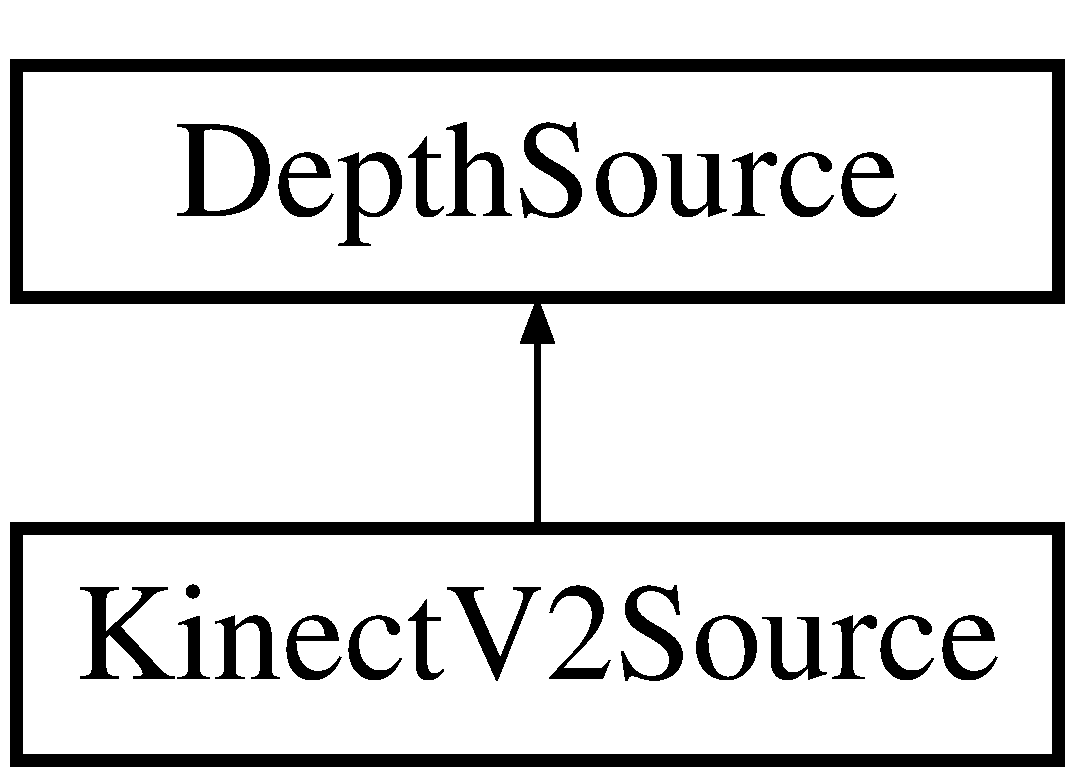
\includegraphics[height=2.000000cm]{class_kinect_v2_source}
\end{center}
\end{figure}
\subsection*{Public Member Functions}
\begin{DoxyCompactItemize}
\item 
\hyperlink{class_kinect_v2_source_aa9c02adca487952da0e24e769e06ea87}{Kinect\+V2\+Source} (\hyperlink{_compression_strategy_8h_a56a83bf6847f4801f4205eb4be237ccf}{Compression} comp)
\begin{DoxyCompactList}\small\item\em Constructor that initializes the I\+Kinect\+Sensor-\/interface. \end{DoxyCompactList}\item 
\hypertarget{class_kinect_v2_source_a9859a72ce30b8b552e90f479bd5609cc}{\hyperlink{class_kinect_v2_source_a9859a72ce30b8b552e90f479bd5609cc}{$\sim$\+Kinect\+V2\+Source} ()}\label{class_kinect_v2_source_a9859a72ce30b8b552e90f479bd5609cc}

\begin{DoxyCompactList}\small\item\em Destructor that releases all the interfaces safely. \end{DoxyCompactList}\item 
\hypertarget{class_kinect_v2_source_aed2fd3bb2b33636b183ff217bf815f38}{void \hyperlink{class_kinect_v2_source_aed2fd3bb2b33636b183ff217bf815f38}{run\+Depth\+Source} ()}\label{class_kinect_v2_source_aed2fd3bb2b33636b183ff217bf815f38}

\begin{DoxyCompactList}\small\item\em Public method which starts the Kinect\+V2-\/interface, which results in the camera filming frames. \end{DoxyCompactList}\item 
\hypertarget{class_kinect_v2_source_a5f492aefe4035084fbb9ca92cc135e1b}{void \hyperlink{class_kinect_v2_source_a5f492aefe4035084fbb9ca92cc135e1b}{stop\+Depth\+Source} ()}\label{class_kinect_v2_source_a5f492aefe4035084fbb9ca92cc135e1b}

\begin{DoxyCompactList}\small\item\em Public method which stops the Kinect\+V2-\/interface, making the camera stop filming. \end{DoxyCompactList}\item 
void \hyperlink{class_kinect_v2_source_a3fa31b0766bb3e9037bb72ef7e4baea7}{save\+Frames\+To\+Directory} (const string \&directory\+\_\+, int N=M\+A\+X\+F\+I\+L\+E\+S)
\begin{DoxyCompactList}\small\item\em Saves a specified number of frames as images in a directory. If the directory already contains frames with the same name they will be overwritten. \end{DoxyCompactList}\end{DoxyCompactItemize}
\subsection*{Additional Inherited Members}


\subsection{Detailed Description}
Class that extends the abstract class \hyperlink{class_depth_source}{Depth\+Source}. Links a Kinect2-\/interface to a private callback method. This method compresses the received frame with a specific \hyperlink{class_compression_strategy}{Compression\+Strategy} and sends it to the backend server using a \hyperlink{class_d_d_s_client}{D\+D\+S\+Client}. 

\subsection{Constructor \& Destructor Documentation}
\hypertarget{class_kinect_v2_source_aa9c02adca487952da0e24e769e06ea87}{\index{Kinect\+V2\+Source@{Kinect\+V2\+Source}!Kinect\+V2\+Source@{Kinect\+V2\+Source}}
\index{Kinect\+V2\+Source@{Kinect\+V2\+Source}!Kinect\+V2\+Source@{Kinect\+V2\+Source}}
\subsubsection[{Kinect\+V2\+Source}]{\setlength{\rightskip}{0pt plus 5cm}Kinect\+V2\+Source\+::\+Kinect\+V2\+Source (
\begin{DoxyParamCaption}
\item[{{\bf Compression}}]{comp}
\end{DoxyParamCaption}
)\hspace{0.3cm}{\ttfamily [inline]}}}\label{class_kinect_v2_source_aa9c02adca487952da0e24e769e06ea87}


Constructor that initializes the I\+Kinect\+Sensor-\/interface. 


\begin{DoxyParams}[1]{Parameters}
\mbox{\tt in}  & {\em comp} & The used \hyperlink{class_compression_strategy}{Compression\+Strategy} (enumerator) \\
\hline
\end{DoxyParams}


\subsection{Member Function Documentation}
\hypertarget{class_kinect_v2_source_a3fa31b0766bb3e9037bb72ef7e4baea7}{\index{Kinect\+V2\+Source@{Kinect\+V2\+Source}!save\+Frames\+To\+Directory@{save\+Frames\+To\+Directory}}
\index{save\+Frames\+To\+Directory@{save\+Frames\+To\+Directory}!Kinect\+V2\+Source@{Kinect\+V2\+Source}}
\subsubsection[{save\+Frames\+To\+Directory}]{\setlength{\rightskip}{0pt plus 5cm}void Kinect\+V2\+Source\+::save\+Frames\+To\+Directory (
\begin{DoxyParamCaption}
\item[{const string \&}]{directory\+\_\+, }
\item[{int}]{N = {\ttfamily MAXFILES}}
\end{DoxyParamCaption}
)\hspace{0.3cm}{\ttfamily [inline]}, {\ttfamily [virtual]}}}\label{class_kinect_v2_source_a3fa31b0766bb3e9037bb72ef7e4baea7}


Saves a specified number of frames as images in a directory. If the directory already contains frames with the same name they will be overwritten. 


\begin{DoxyParams}[1]{Parameters}
\mbox{\tt in}  & {\em directory} & The directory where the frames will be saved \\
\hline
\mbox{\tt in}  & {\em N} & The number of frames that have to be saved \\
\hline
\end{DoxyParams}


Implements \hyperlink{class_depth_source_a9e15edc06570770976693b32ef7c5226}{Depth\+Source}.



The documentation for this class was generated from the following file\+:\begin{DoxyCompactItemize}
\item 
Kinect\+V2\+Source.\+h\end{DoxyCompactItemize}

\hypertarget{struct_kin_fu_l_s_app}{\section{Kin\+Fu\+L\+S\+App Struct Reference}
\label{struct_kin_fu_l_s_app}\index{Kin\+Fu\+L\+S\+App@{Kin\+Fu\+L\+S\+App}}
}
\subsection*{Public Types}
\begin{DoxyCompactItemize}
\item 
\hypertarget{struct_kin_fu_l_s_app_a1bb8f10d28eb4883e70de1c1ae23270d}{enum \{ \\*
{\bfseries P\+C\+D\+\_\+\+B\+I\+N} = 1, 
{\bfseries P\+C\+D\+\_\+\+A\+S\+C\+I\+I} = 2, 
{\bfseries P\+L\+Y} = 3, 
{\bfseries M\+E\+S\+H\+\_\+\+P\+L\+Y} = 7, 
\\*
{\bfseries M\+E\+S\+H\+\_\+\+V\+T\+K} = 8
 \}}\label{struct_kin_fu_l_s_app_a1bb8f10d28eb4883e70de1c1ae23270d}

\end{DoxyCompactItemize}
\subsection*{Public Member Functions}
\begin{DoxyCompactItemize}
\item 
\hypertarget{struct_kin_fu_l_s_app_aaea571898fcf4c7e47c88fea1c994d17}{{\bfseries Kin\+Fu\+L\+S\+App} (pcl\+::\+Grabber \&source, float vsz, float shift\+Distance, int snapshot\+Rate, int total\+\_\+files, int client\+\_\+)}\label{struct_kin_fu_l_s_app_aaea571898fcf4c7e47c88fea1c994d17}

\item 
\hypertarget{struct_kin_fu_l_s_app_a6963b65f27821eaf0b5bf0d8a2ac7720}{void {\bfseries init\+Current\+Frame\+View} ()}\label{struct_kin_fu_l_s_app_a6963b65f27821eaf0b5bf0d8a2ac7720}

\item 
\hypertarget{struct_kin_fu_l_s_app_a004af16f409ebe1bc23cbdd626ee7aba}{void {\bfseries init\+Registration} ()}\label{struct_kin_fu_l_s_app_a004af16f409ebe1bc23cbdd626ee7aba}

\item 
\hypertarget{struct_kin_fu_l_s_app_a6037c71fb3ac44b92a271b64e39dc697}{void {\bfseries toggle\+Color\+Integration} ()}\label{struct_kin_fu_l_s_app_a6037c71fb3ac44b92a271b64e39dc697}

\item 
\hypertarget{struct_kin_fu_l_s_app_aa11b87b7264e0c48b1e1ae1ba617945b}{void {\bfseries toggle\+Independent\+Camera} ()}\label{struct_kin_fu_l_s_app_aa11b87b7264e0c48b1e1ae1ba617945b}

\item 
\hypertarget{struct_kin_fu_l_s_app_aeaa9e6019064691acc6d454592b93c6a}{void {\bfseries toggle\+Evaluation\+Mode} (const string \&eval\+\_\+folder, const string \&match\+\_\+file=string())}\label{struct_kin_fu_l_s_app_aeaa9e6019064691acc6d454592b93c6a}

\item 
\hypertarget{struct_kin_fu_l_s_app_aa2cfc273af83e335934865aec9069892}{void {\bfseries execute} (const Ptr\+Step\+Sz$<$ const unsigned short $>$ \&depth, const Ptr\+Step\+Sz$<$ const pcl\+::gpu\+::kinfu\+L\+S\+::\+Pixel\+R\+G\+B $>$ \&rgb24, bool has\+\_\+data)}\label{struct_kin_fu_l_s_app_aa2cfc273af83e335934865aec9069892}

\item 
\hypertarget{struct_kin_fu_l_s_app_ad99e2511986abfa28694967478457f90}{void {\bfseries source\+\_\+cb1} (const boost\+::shared\+\_\+ptr$<$ openni\+\_\+wrapper\+::\+Depth\+Image $>$ \&depth\+\_\+wrapper)}\label{struct_kin_fu_l_s_app_ad99e2511986abfa28694967478457f90}

\item 
\hypertarget{struct_kin_fu_l_s_app_a45662c8768244fd8b7c5431dacd87881}{void {\bfseries source\+\_\+cb2} (const boost\+::shared\+\_\+ptr$<$ openni\+\_\+wrapper\+::\+Image $>$ \&image\+\_\+wrapper, const boost\+::shared\+\_\+ptr$<$ openni\+\_\+wrapper\+::\+Depth\+Image $>$ \&depth\+\_\+wrapper, float)}\label{struct_kin_fu_l_s_app_a45662c8768244fd8b7c5431dacd87881}

\item 
\hypertarget{struct_kin_fu_l_s_app_adf886de05d76766c51d6079f8b15db9c}{void {\bfseries source\+\_\+cb3} (const pcl\+::\+Point\+Cloud$<$ pcl\+::\+Point\+X\+Y\+Z\+R\+G\+B\+A $>$\+::Const\+Ptr \&D\+C3)}\label{struct_kin_fu_l_s_app_adf886de05d76766c51d6079f8b15db9c}

\item 
\hypertarget{struct_kin_fu_l_s_app_a53d96a404961fa08811f2b6d48920782}{void {\bfseries start\+Main\+Loop} (bool triggered\+\_\+capture)}\label{struct_kin_fu_l_s_app_a53d96a404961fa08811f2b6d48920782}

\item 
\hypertarget{struct_kin_fu_l_s_app_a1d855097fedbba14e864022032cc9515}{void {\bfseries write\+Cloud} (int format) const }\label{struct_kin_fu_l_s_app_a1d855097fedbba14e864022032cc9515}

\item 
\hypertarget{struct_kin_fu_l_s_app_acec9efc09fa50d35e65b32d221e01f57}{void {\bfseries write\+Mesh} (int format) const }\label{struct_kin_fu_l_s_app_acec9efc09fa50d35e65b32d221e01f57}

\item 
\hypertarget{struct_kin_fu_l_s_app_a4c5fff246a4aaf1b703bf276c3daf51b}{void {\bfseries print\+Help} ()}\label{struct_kin_fu_l_s_app_a4c5fff246a4aaf1b703bf276c3daf51b}

\end{DoxyCompactItemize}
\subsection*{Static Public Member Functions}
\begin{DoxyCompactItemize}
\item 
\hypertarget{struct_kin_fu_l_s_app_ada8919c6a7cc2389c420a132b066f818}{static void {\bfseries keyboard\+\_\+callback} (const visualization\+::\+Keyboard\+Event \&e, void $\ast$cookie)}\label{struct_kin_fu_l_s_app_ada8919c6a7cc2389c420a132b066f818}

\end{DoxyCompactItemize}
\subsection*{Public Attributes}
\begin{DoxyCompactItemize}
\item 
\hypertarget{struct_kin_fu_l_s_app_a1c5769a12e06dc3912d6584523bd71d0}{bool {\bfseries exit\+\_\+}}\label{struct_kin_fu_l_s_app_a1c5769a12e06dc3912d6584523bd71d0}

\item 
\hypertarget{struct_kin_fu_l_s_app_aba97d2165d7108bde30af7e5805bd6bd}{bool {\bfseries scan\+\_\+}}\label{struct_kin_fu_l_s_app_aba97d2165d7108bde30af7e5805bd6bd}

\item 
\hypertarget{struct_kin_fu_l_s_app_a62ee9b37fa531f4839ecdf64310cd4d0}{bool {\bfseries scan\+\_\+mesh\+\_\+}}\label{struct_kin_fu_l_s_app_a62ee9b37fa531f4839ecdf64310cd4d0}

\item 
\hypertarget{struct_kin_fu_l_s_app_ab2716c9664a729f6802c379ef085d5b7}{bool {\bfseries scan\+\_\+volume\+\_\+}}\label{struct_kin_fu_l_s_app_ab2716c9664a729f6802c379ef085d5b7}

\item 
\hypertarget{struct_kin_fu_l_s_app_adff42afe85cd544473eb19153d5b9b61}{bool {\bfseries independent\+\_\+camera\+\_\+}}\label{struct_kin_fu_l_s_app_adff42afe85cd544473eb19153d5b9b61}

\item 
\hypertarget{struct_kin_fu_l_s_app_a1dcc90b89fc50705c8289d204205b2d7}{int {\bfseries frame\+\_\+counter\+\_\+}}\label{struct_kin_fu_l_s_app_a1dcc90b89fc50705c8289d204205b2d7}

\item 
\hypertarget{struct_kin_fu_l_s_app_aaf183373085a0f83145b45cacf0b26f0}{bool {\bfseries enable\+\_\+texture\+\_\+extraction\+\_\+}}\label{struct_kin_fu_l_s_app_aaf183373085a0f83145b45cacf0b26f0}

\item 
\hypertarget{struct_kin_fu_l_s_app_a539b7cb75153a3e53dd2a25f1756b900}{pcl\+::kinfu\+L\+S\+::\+Screenshot\+Manager {\bfseries screenshot\+\_\+manager\+\_\+}}\label{struct_kin_fu_l_s_app_a539b7cb75153a3e53dd2a25f1756b900}

\item 
\hypertarget{struct_kin_fu_l_s_app_a8a95aa8eda0d5bd23bb3557e39948600}{int {\bfseries snapshot\+\_\+rate\+\_\+}}\label{struct_kin_fu_l_s_app_a8a95aa8eda0d5bd23bb3557e39948600}

\item 
\hypertarget{struct_kin_fu_l_s_app_aca5edae888ae830f27a3313a5bdb47c8}{int {\bfseries total\+\_\+files\+\_\+}}\label{struct_kin_fu_l_s_app_aca5edae888ae830f27a3313a5bdb47c8}

\item 
\hypertarget{struct_kin_fu_l_s_app_ad5ccfa059d15469a0d31de819db76808}{int {\bfseries current\+\_\+file}}\label{struct_kin_fu_l_s_app_ad5ccfa059d15469a0d31de819db76808}

\item 
\hypertarget{struct_kin_fu_l_s_app_ad1df9eccb3a3299f6566612ef1597664}{int {\bfseries client}}\label{struct_kin_fu_l_s_app_ad1df9eccb3a3299f6566612ef1597664}

\item 
\hypertarget{struct_kin_fu_l_s_app_a8b0673281ed574962e3a1b6c5eb58cc4}{bool {\bfseries registration\+\_\+}}\label{struct_kin_fu_l_s_app_a8b0673281ed574962e3a1b6c5eb58cc4}

\item 
\hypertarget{struct_kin_fu_l_s_app_aa6574f198ee47082a329a558001424ba}{bool {\bfseries integrate\+\_\+colors\+\_\+}}\label{struct_kin_fu_l_s_app_aa6574f198ee47082a329a558001424ba}

\item 
\hypertarget{struct_kin_fu_l_s_app_afe09648059b3ab2c3316bf551016cb1e}{bool {\bfseries pcd\+\_\+source\+\_\+}}\label{struct_kin_fu_l_s_app_afe09648059b3ab2c3316bf551016cb1e}

\item 
\hypertarget{struct_kin_fu_l_s_app_a690e662ddd208bd6af2518afcc6d3964}{float {\bfseries focal\+\_\+length\+\_\+}}\label{struct_kin_fu_l_s_app_a690e662ddd208bd6af2518afcc6d3964}

\item 
\hypertarget{struct_kin_fu_l_s_app_a3c6165d4b78a7f150a3574e5378a19eb}{pcl\+::\+Grabber \& {\bfseries capture\+\_\+}}\label{struct_kin_fu_l_s_app_a3c6165d4b78a7f150a3574e5378a19eb}

\item 
\hypertarget{struct_kin_fu_l_s_app_a1e5eb5ce36cf1f4db0a75b2d306cd8a2}{Kinfu\+Tracker $\ast$ {\bfseries kinfu\+\_\+}}\label{struct_kin_fu_l_s_app_a1e5eb5ce36cf1f4db0a75b2d306cd8a2}

\item 
\hypertarget{struct_kin_fu_l_s_app_a5484e646b6be4441a2a094b42fff8e2d}{\hyperlink{struct_scene_cloud_view}{Scene\+Cloud\+View} {\bfseries scene\+\_\+cloud\+\_\+view\+\_\+}}\label{struct_kin_fu_l_s_app_a5484e646b6be4441a2a094b42fff8e2d}

\item 
\hypertarget{struct_kin_fu_l_s_app_ab70151a58a620d9da106528e2d4328e9}{\hyperlink{struct_image_view}{Image\+View} {\bfseries image\+\_\+view\+\_\+}}\label{struct_kin_fu_l_s_app_ab70151a58a620d9da106528e2d4328e9}

\item 
\hypertarget{struct_kin_fu_l_s_app_af5566b10bf5cb0b62fb5f7fb7ad89134}{boost\+::shared\+\_\+ptr\\*
$<$ \hyperlink{struct_current_frame_cloud_view}{Current\+Frame\+Cloud\+View} $>$ {\bfseries current\+\_\+frame\+\_\+cloud\+\_\+view\+\_\+}}\label{struct_kin_fu_l_s_app_af5566b10bf5cb0b62fb5f7fb7ad89134}

\item 
\hypertarget{struct_kin_fu_l_s_app_a6ffc741a4ccd7cd922113d02d4a18570}{Kinfu\+Tracker\+::\+Depth\+Map {\bfseries depth\+\_\+device\+\_\+}}\label{struct_kin_fu_l_s_app_a6ffc741a4ccd7cd922113d02d4a18570}

\item 
\hypertarget{struct_kin_fu_l_s_app_ab1a30ac44ea215a0e238d356c3799417}{pcl\+::\+Point\+Cloud\\*
$<$ pcl\+::\+Point\+X\+Y\+Z\+I $>$\+::Ptr {\bfseries tsdf\+\_\+cloud\+\_\+ptr\+\_\+}}\label{struct_kin_fu_l_s_app_ab1a30ac44ea215a0e238d356c3799417}

\item 
\hypertarget{struct_kin_fu_l_s_app_a17f5ee34dd0d278366798f700cf0a8ba}{Evaluation\+::\+Ptr {\bfseries evaluation\+\_\+ptr\+\_\+}}\label{struct_kin_fu_l_s_app_a17f5ee34dd0d278366798f700cf0a8ba}

\item 
\hypertarget{struct_kin_fu_l_s_app_a2efa66f544a6e297931b0149cbd386a6}{boost\+::mutex {\bfseries data\+\_\+ready\+\_\+mutex\+\_\+}}\label{struct_kin_fu_l_s_app_a2efa66f544a6e297931b0149cbd386a6}

\item 
\hypertarget{struct_kin_fu_l_s_app_ae7606382c03b67819472d32dd17e5754}{boost\+::condition\+\_\+variable {\bfseries data\+\_\+ready\+\_\+cond\+\_\+}}\label{struct_kin_fu_l_s_app_ae7606382c03b67819472d32dd17e5754}

\item 
\hypertarget{struct_kin_fu_l_s_app_af97d98a16c6645357316a2ce5ca08c11}{std\+::vector\\*
$<$ pcl\+::gpu\+::kinfu\+L\+S\+::\+Pixel\+R\+G\+B $>$ {\bfseries source\+\_\+image\+\_\+data\+\_\+}}\label{struct_kin_fu_l_s_app_af97d98a16c6645357316a2ce5ca08c11}

\item 
\hypertarget{struct_kin_fu_l_s_app_a3cf45ae0744e4fe782d17b5445226652}{std\+::vector$<$ unsigned short $>$ {\bfseries source\+\_\+depth\+\_\+data\+\_\+}}\label{struct_kin_fu_l_s_app_a3cf45ae0744e4fe782d17b5445226652}

\item 
\hypertarget{struct_kin_fu_l_s_app_af93fe53119a99a3d17b419c4bfb811f3}{Ptr\+Step\+Sz$<$ const unsigned short $>$ {\bfseries depth\+\_\+}}\label{struct_kin_fu_l_s_app_af93fe53119a99a3d17b419c4bfb811f3}

\item 
\hypertarget{struct_kin_fu_l_s_app_a0a783d5d6f1b99c22a226e68679c5dfa}{Ptr\+Step\+Sz$<$ const \\*
pcl\+::gpu\+::kinfu\+L\+S\+::\+Pixel\+R\+G\+B $>$ {\bfseries rgb24\+\_\+}}\label{struct_kin_fu_l_s_app_a0a783d5d6f1b99c22a226e68679c5dfa}

\item 
\hypertarget{struct_kin_fu_l_s_app_a1f73527db56daf7519e0028708b02656}{Eigen\+::\+Affine3f {\bfseries delta\+\_\+lost\+\_\+pose\+\_\+}}\label{struct_kin_fu_l_s_app_a1f73527db56daf7519e0028708b02656}

\item 
\hypertarget{struct_kin_fu_l_s_app_a1b0459479f1f21f94e344b7cffbb2796}{bool {\bfseries was\+\_\+lost\+\_\+}}\label{struct_kin_fu_l_s_app_a1b0459479f1f21f94e344b7cffbb2796}

\item 
\hypertarget{struct_kin_fu_l_s_app_ab1242b012cf2272bcb7921716d2d2f59}{int {\bfseries time\+\_\+ms\+\_\+}}\label{struct_kin_fu_l_s_app_ab1242b012cf2272bcb7921716d2d2f59}

\end{DoxyCompactItemize}


The documentation for this struct was generated from the following file\+:\begin{DoxyCompactItemize}
\item 
kinfu\+L\+S\+\_\+app.\+cpp\end{DoxyCompactItemize}

\hypertarget{class_kinfu_processor}{\section{Kinfu\+Processor Class Reference}
\label{class_kinfu_processor}\index{Kinfu\+Processor@{Kinfu\+Processor}}
}


Class that processes saved pointclouds and converts them into a world pointcloud.  




{\ttfamily \#include $<$Kinfu\+Processor.\+h$>$}

\subsection*{Public Member Functions}
\begin{DoxyCompactItemize}
\item 
\hypertarget{class_kinfu_processor_a17125ce0336fab773e0460055997ef9e}{int {\bfseries Process\+Kinfu\+Client} (const int \&i, char $\ast$\&worldbuffer, int \&size)}\label{class_kinfu_processor_a17125ce0336fab773e0460055997ef9e}

\end{DoxyCompactItemize}


\subsection{Detailed Description}
Class that processes saved pointclouds and converts them into a world pointcloud. 

The documentation for this class was generated from the following file\+:\begin{DoxyCompactItemize}
\item 
Kinfu\+Processor.\+h\end{DoxyCompactItemize}

\hypertarget{class_limited_queue}{\section{Limited\+Queue Class Reference}
\label{class_limited_queue}\index{Limited\+Queue@{Limited\+Queue}}
}


Class that acts as a queue with a limited size for Frames.  




{\ttfamily \#include $<$D\+D\+S\+Client.\+h$>$}

\subsection*{Public Member Functions}
\begin{DoxyCompactItemize}
\item 
\hypertarget{class_limited_queue_a8662be2f2126546e2cc35a0c1a3288b5}{{\bfseries Limited\+Queue} (int max=M\+A\+X\+\_\+\+Q\+U\+E\+U\+E)}\label{class_limited_queue_a8662be2f2126546e2cc35a0c1a3288b5}

\item 
\hypertarget{class_limited_queue_a0ded894c203bf8d4ce6fd2a6266b8dee}{void {\bfseries push} (\hyperlink{struct_frame}{Frame} \&f)}\label{class_limited_queue_a0ded894c203bf8d4ce6fd2a6266b8dee}

\item 
\hypertarget{class_limited_queue_abe2132dfba699ca062d2d4b2e6a15172}{void {\bfseries reduce\+Queue} ()}\label{class_limited_queue_abe2132dfba699ca062d2d4b2e6a15172}

\item 
\hypertarget{class_limited_queue_aab4b64ea7239ce1df3e92c32e69f36bc}{\hyperlink{struct_frame}{Frame} {\bfseries front} ()}\label{class_limited_queue_aab4b64ea7239ce1df3e92c32e69f36bc}

\item 
\hypertarget{class_limited_queue_a1ca6b83ee0ac44d9ffa4e903c4dfa0e3}{void {\bfseries pop} ()}\label{class_limited_queue_a1ca6b83ee0ac44d9ffa4e903c4dfa0e3}

\item 
\hypertarget{class_limited_queue_a01187e2fcfa91ca29fda18f6d913e108}{int {\bfseries size} ()}\label{class_limited_queue_a01187e2fcfa91ca29fda18f6d913e108}

\item 
\hypertarget{class_limited_queue_ab08d0ed1c58715dc9b6a165557591257}{int {\bfseries remaining\+Halved} ()}\label{class_limited_queue_ab08d0ed1c58715dc9b6a165557591257}

\end{DoxyCompactItemize}


\subsection{Detailed Description}
Class that acts as a queue with a limited size for Frames. 

The documentation for this class was generated from the following file\+:\begin{DoxyCompactItemize}
\item 
\hyperlink{_d_d_s_client_8h}{D\+D\+S\+Client.\+h}\end{DoxyCompactItemize}

\hypertarget{structmem__encode}{\section{mem\+\_\+encode Struct Reference}
\label{structmem__encode}\index{mem\+\_\+encode@{mem\+\_\+encode}}
}
\subsection*{Public Attributes}
\begin{DoxyCompactItemize}
\item 
\hypertarget{structmem__encode_a70f5426618e93ea6cb7259e8df552610}{char $\ast$ {\bfseries buffer}}\label{structmem__encode_a70f5426618e93ea6cb7259e8df552610}

\item 
\hypertarget{structmem__encode_adfd242fbd7f1bed163deaa6912f21081}{size\+\_\+t {\bfseries size}}\label{structmem__encode_adfd242fbd7f1bed163deaa6912f21081}

\end{DoxyCompactItemize}


The documentation for this struct was generated from the following file\+:\begin{DoxyCompactItemize}
\item 
\hyperlink{_p_n_g_strategy_8h}{P\+N\+G\+Strategy.\+h}\end{DoxyCompactItemize}

\hypertarget{structmy__source__mgr}{\section{my\+\_\+source\+\_\+mgr Struct Reference}
\label{structmy__source__mgr}\index{my\+\_\+source\+\_\+mgr@{my\+\_\+source\+\_\+mgr}}
}
\subsection*{Public Attributes}
\begin{DoxyCompactItemize}
\item 
\hypertarget{structmy__source__mgr_a8572f33f87bec948592001edea12680f}{struct jpeg\+\_\+source\+\_\+mgr {\bfseries pub}}\label{structmy__source__mgr_a8572f33f87bec948592001edea12680f}

\item 
\hypertarget{structmy__source__mgr_ad9a24935cf19bd9dc1ace874a11e886d}{const J\+O\+C\+T\+E\+T $\ast$ {\bfseries data}}\label{structmy__source__mgr_ad9a24935cf19bd9dc1ace874a11e886d}

\item 
\hypertarget{structmy__source__mgr_ad6ba4e08165f32e64469f754d4671bd9}{size\+\_\+t {\bfseries len}}\label{structmy__source__mgr_ad6ba4e08165f32e64469f754d4671bd9}

\end{DoxyCompactItemize}


The documentation for this struct was generated from the following files\+:\begin{DoxyCompactItemize}
\item 
\hyperlink{_j_p_e_g_decompression_8h}{J\+P\+E\+G\+Decompression.\+h}\item 
\hyperlink{_j_p_e_g_strategy_8h}{J\+P\+E\+G\+Strategy.\+h}\end{DoxyCompactItemize}

\hypertarget{class_open_n_i_source}{\section{Open\+N\+I\+Source Class Reference}
\label{class_open_n_i_source}\index{Open\+N\+I\+Source@{Open\+N\+I\+Source}}
}


Class that extends the abstract class \hyperlink{class_depth_source}{Depth\+Source}. Links an Open\+N\+I Grabber-\/interface to a private callback method. This method compresses the received frame with a specific \hyperlink{class_compression_strategy}{Compression\+Strategy} and sends it to the backend server using a \hyperlink{class_d_d_s_client}{D\+D\+S\+Client}.  




{\ttfamily \#include $<$Open\+N\+I\+Source.\+h$>$}

Inheritance diagram for Open\+N\+I\+Source\+:\begin{figure}[H]
\begin{center}
\leavevmode
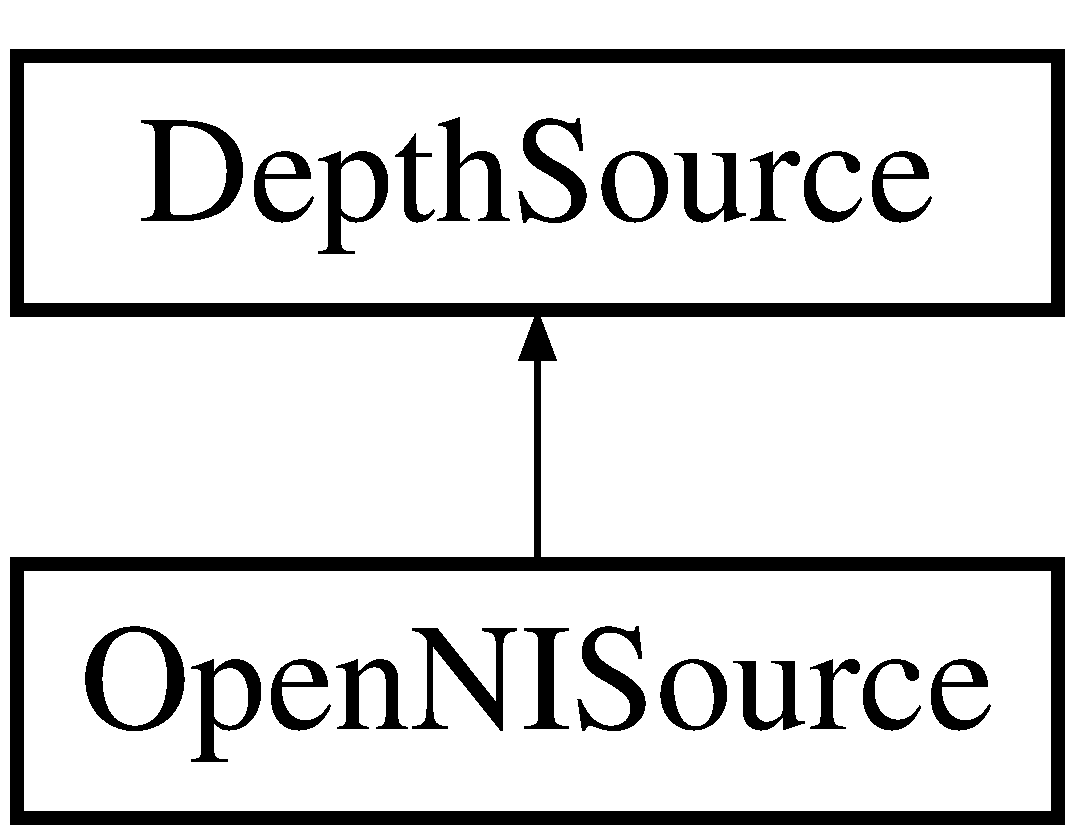
\includegraphics[height=2.000000cm]{class_open_n_i_source}
\end{center}
\end{figure}
\subsection*{Public Member Functions}
\begin{DoxyCompactItemize}
\item 
\hypertarget{class_open_n_i_source_ad7c59826245812024bee0a541f948c91}{\hyperlink{class_open_n_i_source_ad7c59826245812024bee0a541f948c91}{Open\+N\+I\+Source} (\hyperlink{_compression_strategy_8h_a56a83bf6847f4801f4205eb4be237ccf}{Compression} comp)}\label{class_open_n_i_source_ad7c59826245812024bee0a541f948c91}

\begin{DoxyCompactList}\small\item\em Constructor that links the Grabber-\/interface to a private callback method. \end{DoxyCompactList}\item 
\hypertarget{class_open_n_i_source_ad0d3202f60119589e1d8b5ba94e49e59}{void \hyperlink{class_open_n_i_source_ad0d3202f60119589e1d8b5ba94e49e59}{run\+Depth\+Source} ()}\label{class_open_n_i_source_ad0d3202f60119589e1d8b5ba94e49e59}

\begin{DoxyCompactList}\small\item\em Public method which starts the Open\+N\+I Grabber-\/interface, which results in the camera filming frames. \end{DoxyCompactList}\item 
\hypertarget{class_open_n_i_source_aa92ab17d6933c1f5447f0f581815a4e6}{void \hyperlink{class_open_n_i_source_aa92ab17d6933c1f5447f0f581815a4e6}{stop\+Depth\+Source} ()}\label{class_open_n_i_source_aa92ab17d6933c1f5447f0f581815a4e6}

\begin{DoxyCompactList}\small\item\em Public method which stops the Grabber-\/interface, making the camera stop filming. \end{DoxyCompactList}\item 
void \hyperlink{class_open_n_i_source_a2d6f642492a63ebb1cef48e927d52a06}{save\+Frames\+To\+Directory} (const string \&directory\+\_\+, int N=M\+A\+X\+F\+I\+L\+E\+S)
\begin{DoxyCompactList}\small\item\em Saves a specified number of frames as images in a directory. \end{DoxyCompactList}\end{DoxyCompactItemize}
\subsection*{Additional Inherited Members}


\subsection{Detailed Description}
Class that extends the abstract class \hyperlink{class_depth_source}{Depth\+Source}. Links an Open\+N\+I Grabber-\/interface to a private callback method. This method compresses the received frame with a specific \hyperlink{class_compression_strategy}{Compression\+Strategy} and sends it to the backend server using a \hyperlink{class_d_d_s_client}{D\+D\+S\+Client}. 

\subsection{Member Function Documentation}
\hypertarget{class_open_n_i_source_a2d6f642492a63ebb1cef48e927d52a06}{\index{Open\+N\+I\+Source@{Open\+N\+I\+Source}!save\+Frames\+To\+Directory@{save\+Frames\+To\+Directory}}
\index{save\+Frames\+To\+Directory@{save\+Frames\+To\+Directory}!Open\+N\+I\+Source@{Open\+N\+I\+Source}}
\subsubsection[{save\+Frames\+To\+Directory}]{\setlength{\rightskip}{0pt plus 5cm}void Open\+N\+I\+Source\+::save\+Frames\+To\+Directory (
\begin{DoxyParamCaption}
\item[{const string \&}]{directory\+\_\+, }
\item[{int}]{N = {\ttfamily MAXFILES}}
\end{DoxyParamCaption}
)\hspace{0.3cm}{\ttfamily [inline]}, {\ttfamily [virtual]}}}\label{class_open_n_i_source_a2d6f642492a63ebb1cef48e927d52a06}


Saves a specified number of frames as images in a directory. 


\begin{DoxyParams}[1]{Parameters}
\mbox{\tt in}  & {\em directory} & The directory where the frames will be saved \\
\hline
\mbox{\tt in}  & {\em N} & The number of frames that have to be saved \\
\hline
\end{DoxyParams}


Implements \hyperlink{class_depth_source_a9e15edc06570770976693b32ef7c5226}{Depth\+Source}.



The documentation for this class was generated from the following file\+:\begin{DoxyCompactItemize}
\item 
\hyperlink{_open_n_i_source_8h}{Open\+N\+I\+Source.\+h}\end{DoxyCompactItemize}

\hypertarget{class_p_n_g_strategy}{\section{P\+N\+G\+Strategy Class Reference}
\label{class_p_n_g_strategy}\index{P\+N\+G\+Strategy@{P\+N\+G\+Strategy}}
}


Class that extends the abstract class \hyperlink{class_compression_strategy}{Compression\+Strategy}. Offers the functionality to compress a depth matrix to a 16-\/bit P\+N\+G-\/image. T\+O\+D\+O.  




{\ttfamily \#include $<$P\+N\+G\+Strategy.\+h$>$}

Inheritance diagram for P\+N\+G\+Strategy\+:\begin{figure}[H]
\begin{center}
\leavevmode
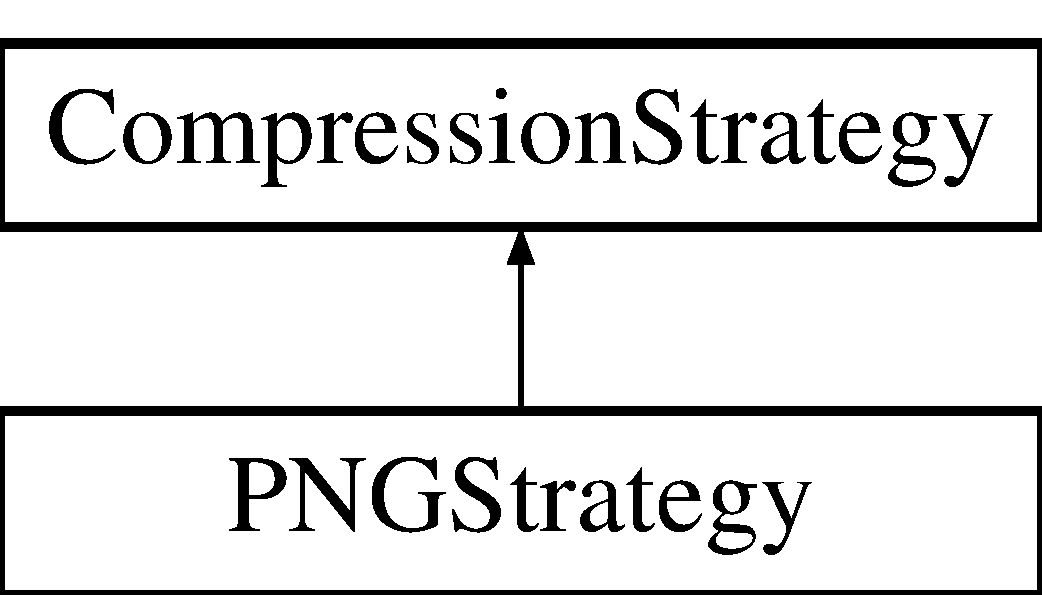
\includegraphics[height=2.000000cm]{class_p_n_g_strategy}
\end{center}
\end{figure}
\subsection*{Public Member Functions}
\begin{DoxyCompactItemize}
\item 
void \hyperlink{class_p_n_g_strategy_aaa542a51c70ede4b82facb66d9ff9ec2}{compress\+\_\+depth\+\_\+to\+\_\+image} (const int \&x\+Resolution, const int \&y\+Resolution, short $\ast$depth\+Data, unsigned char $\ast$\&out\+\_\+buffer\+\_\+, int \&n\+Bytes)
\begin{DoxyCompactList}\small\item\em Public method that offers the functionality to compress a depth matrix to a 16-\/bit P\+N\+G-\/image. \end{DoxyCompactList}\item 
void \hyperlink{class_p_n_g_strategy_a170b89ef5e216f9166d80916d3efe1b0}{decompress\+\_\+image\+\_\+to\+\_\+depth} (const int \&x\+Resolution, const int \&y\+Resolution, short $\ast$\&depth\+Data, unsigned char $\ast$image, int \&n\+Bytes)
\begin{DoxyCompactList}\small\item\em Public method that offers the functionality to decompress a 12-\/bit J\+P\+E\+G-\/image to a depth matrix. \end{DoxyCompactList}\end{DoxyCompactItemize}


\subsection{Detailed Description}
Class that extends the abstract class \hyperlink{class_compression_strategy}{Compression\+Strategy}. Offers the functionality to compress a depth matrix to a 16-\/bit P\+N\+G-\/image. T\+O\+D\+O. 

\subsection{Member Function Documentation}
\hypertarget{class_p_n_g_strategy_aaa542a51c70ede4b82facb66d9ff9ec2}{\index{P\+N\+G\+Strategy@{P\+N\+G\+Strategy}!compress\+\_\+depth\+\_\+to\+\_\+image@{compress\+\_\+depth\+\_\+to\+\_\+image}}
\index{compress\+\_\+depth\+\_\+to\+\_\+image@{compress\+\_\+depth\+\_\+to\+\_\+image}!P\+N\+G\+Strategy@{P\+N\+G\+Strategy}}
\subsubsection[{compress\+\_\+depth\+\_\+to\+\_\+image}]{\setlength{\rightskip}{0pt plus 5cm}void P\+N\+G\+Strategy\+::compress\+\_\+depth\+\_\+to\+\_\+image (
\begin{DoxyParamCaption}
\item[{const int \&}]{x\+Resolution, }
\item[{const int \&}]{y\+Resolution, }
\item[{short $\ast$}]{depth\+Data, }
\item[{unsigned char $\ast$\&}]{out\+\_\+buffer\+\_\+, }
\item[{int \&}]{n\+Bytes}
\end{DoxyParamCaption}
)\hspace{0.3cm}{\ttfamily [inline]}, {\ttfamily [virtual]}}}\label{class_p_n_g_strategy_aaa542a51c70ede4b82facb66d9ff9ec2}


Public method that offers the functionality to compress a depth matrix to a 16-\/bit P\+N\+G-\/image. 


\begin{DoxyParams}[1]{Parameters}
\mbox{\tt in}  & {\em x\+Resolution} & The horizontal resolution of the used camera \\
\hline
\mbox{\tt in}  & {\em y\+Resolution} & The vertical resolution of the used camera \\
\hline
\mbox{\tt in}  & {\em depth\+Data} & A pointer to a depthmatrix containing the depth data \\
\hline
\mbox{\tt out}  & {\em out\+\_\+buffer} & A pointer to a databuffer containing the compressed image \\
\hline
\mbox{\tt out}  & {\em n\+Bytes} & The size of the out\+\_\+buffer in bytes \\
\hline
\end{DoxyParams}


Implements \hyperlink{class_compression_strategy_a5124d2838fc7d8c769a34744f21602f4}{Compression\+Strategy}.

\hypertarget{class_p_n_g_strategy_a170b89ef5e216f9166d80916d3efe1b0}{\index{P\+N\+G\+Strategy@{P\+N\+G\+Strategy}!decompress\+\_\+image\+\_\+to\+\_\+depth@{decompress\+\_\+image\+\_\+to\+\_\+depth}}
\index{decompress\+\_\+image\+\_\+to\+\_\+depth@{decompress\+\_\+image\+\_\+to\+\_\+depth}!P\+N\+G\+Strategy@{P\+N\+G\+Strategy}}
\subsubsection[{decompress\+\_\+image\+\_\+to\+\_\+depth}]{\setlength{\rightskip}{0pt plus 5cm}void P\+N\+G\+Strategy\+::decompress\+\_\+image\+\_\+to\+\_\+depth (
\begin{DoxyParamCaption}
\item[{const int \&}]{x\+Resolution, }
\item[{const int \&}]{y\+Resolution, }
\item[{short $\ast$\&}]{depth\+Data, }
\item[{unsigned char $\ast$}]{image, }
\item[{int \&}]{n\+Bytes}
\end{DoxyParamCaption}
)\hspace{0.3cm}{\ttfamily [inline]}, {\ttfamily [virtual]}}}\label{class_p_n_g_strategy_a170b89ef5e216f9166d80916d3efe1b0}


Public method that offers the functionality to decompress a 12-\/bit J\+P\+E\+G-\/image to a depth matrix. 


\begin{DoxyParams}[1]{Parameters}
\mbox{\tt in}  & {\em x\+Resolution} & The horizontal resolution of the used camera \\
\hline
\mbox{\tt in}  & {\em y\+Resolution} & The vertical resolution of the used camera \\
\hline
\mbox{\tt in}  & {\em depth\+Data} & A pointer to a depthmatrix containing the depth data \\
\hline
\mbox{\tt out}  & {\em image} & A pointer to a databuffer containing the compressed image \\
\hline
\mbox{\tt out}  & {\em n\+Bytes} & The size of the image in bytes \\
\hline
\end{DoxyParams}


Implements \hyperlink{class_compression_strategy}{Compression\+Strategy}.



The documentation for this class was generated from the following file\+:\begin{DoxyCompactItemize}
\item 
\hyperlink{_p_n_g_strategy_8h}{P\+N\+G\+Strategy.\+h}\end{DoxyCompactItemize}

\hypertarget{struct_sampled_scope_time}{\section{Sampled\+Scope\+Time Struct Reference}
\label{struct_sampled_scope_time}\index{Sampled\+Scope\+Time@{Sampled\+Scope\+Time}}
}
Inheritance diagram for Sampled\+Scope\+Time\+:\begin{figure}[H]
\begin{center}
\leavevmode
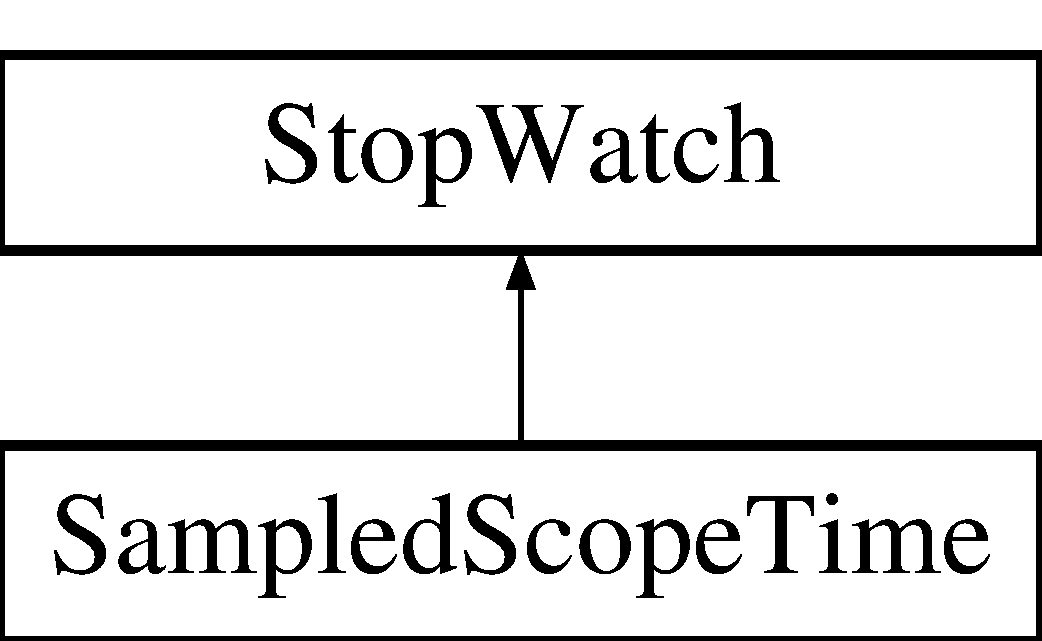
\includegraphics[height=2.000000cm]{struct_sampled_scope_time}
\end{center}
\end{figure}
\subsection*{Public Types}
\begin{DoxyCompactItemize}
\item 
\hypertarget{struct_sampled_scope_time_a3f7d1737ccbbe54c16f585f47affeb7d}{enum \{ {\bfseries E\+A\+C\+H} = 33
 \}}\label{struct_sampled_scope_time_a3f7d1737ccbbe54c16f585f47affeb7d}

\end{DoxyCompactItemize}
\subsection*{Public Member Functions}
\begin{DoxyCompactItemize}
\item 
\hypertarget{struct_sampled_scope_time_acb560b4832e10ccb05ed6764c21e0274}{{\bfseries Sampled\+Scope\+Time} (int \&time\+\_\+ms)}\label{struct_sampled_scope_time_acb560b4832e10ccb05ed6764c21e0274}

\end{DoxyCompactItemize}


The documentation for this struct was generated from the following file\+:\begin{DoxyCompactItemize}
\item 
kinfu\+L\+S\+\_\+app.\+cpp\end{DoxyCompactItemize}

\hypertarget{struct_scene_cloud_view}{\section{Scene\+Cloud\+View Struct Reference}
\label{struct_scene_cloud_view}\index{Scene\+Cloud\+View@{Scene\+Cloud\+View}}
}
\subsection*{Public Types}
\begin{DoxyCompactItemize}
\item 
\hypertarget{struct_scene_cloud_view_a0296162bfcc96b5b8af6b4dd11cf5b34}{enum \{ {\bfseries G\+P\+U\+\_\+\+Connected6} = 0, 
{\bfseries C\+P\+U\+\_\+\+Connected6} = 1, 
{\bfseries C\+P\+U\+\_\+\+Connected26} = 2
 \}}\label{struct_scene_cloud_view_a0296162bfcc96b5b8af6b4dd11cf5b34}

\end{DoxyCompactItemize}
\subsection*{Public Member Functions}
\begin{DoxyCompactItemize}
\item 
\hypertarget{struct_scene_cloud_view_a7cd6f6839d610c4653847b3b1c34880c}{void {\bfseries draw\+Camera} (Eigen\+::\+Affine3f \&pose, const string \&name, double r, double g, double b)}\label{struct_scene_cloud_view_a7cd6f6839d610c4653847b3b1c34880c}

\item 
\hypertarget{struct_scene_cloud_view_aa62c8ada85b5cb6888f5826d20c1bce7}{void {\bfseries remove\+Camera} (const string \&name)}\label{struct_scene_cloud_view_aa62c8ada85b5cb6888f5826d20c1bce7}

\item 
\hypertarget{struct_scene_cloud_view_aa13f0f30c1f98c7996c73be747716603}{void {\bfseries display\+I\+C\+P\+State} (Kinfu\+Tracker \&kinfu, bool was\+\_\+lost\+\_\+)}\label{struct_scene_cloud_view_aa13f0f30c1f98c7996c73be747716603}

\item 
\hypertarget{struct_scene_cloud_view_abf6b5dc76d3dd5b749f4678a396a1dcb}{void {\bfseries show} (Kinfu\+Tracker \&kinfu, bool integrate\+\_\+colors)}\label{struct_scene_cloud_view_abf6b5dc76d3dd5b749f4678a396a1dcb}

\item 
\hypertarget{struct_scene_cloud_view_ad1643724f930b5ad0e1421c9315be25b}{void {\bfseries toggle\+Cube} (const Eigen\+::\+Vector3f \&size)}\label{struct_scene_cloud_view_ad1643724f930b5ad0e1421c9315be25b}

\item 
\hypertarget{struct_scene_cloud_view_af9ba10707d975a4217188fe27f4674c7}{void {\bfseries toggle\+Extraction\+Mode} ()}\label{struct_scene_cloud_view_af9ba10707d975a4217188fe27f4674c7}

\item 
\hypertarget{struct_scene_cloud_view_a4a905792b1bc9fbce3f7cffe68e6acad}{void {\bfseries toggle\+Normals} ()}\label{struct_scene_cloud_view_a4a905792b1bc9fbce3f7cffe68e6acad}

\item 
\hypertarget{struct_scene_cloud_view_aa424f942a142f1c0523529cf936ca6c8}{void {\bfseries clear\+Clouds} (bool print\+\_\+message=false)}\label{struct_scene_cloud_view_aa424f942a142f1c0523529cf936ca6c8}

\item 
\hypertarget{struct_scene_cloud_view_ac898c36f22b4ab497377682305cd99e4}{void {\bfseries show\+Mesh} (Kinfu\+Tracker \&kinfu, bool)}\label{struct_scene_cloud_view_ac898c36f22b4ab497377682305cd99e4}

\end{DoxyCompactItemize}
\subsection*{Public Attributes}
\begin{DoxyCompactItemize}
\item 
\hypertarget{struct_scene_cloud_view_ac613a3b8c4076cf63e5ae8bd9a18276e}{int {\bfseries extraction\+\_\+mode\+\_\+}}\label{struct_scene_cloud_view_ac613a3b8c4076cf63e5ae8bd9a18276e}

\item 
\hypertarget{struct_scene_cloud_view_a2cf11e520aecc6ff80d537dbab502010}{bool {\bfseries compute\+\_\+normals\+\_\+}}\label{struct_scene_cloud_view_a2cf11e520aecc6ff80d537dbab502010}

\item 
\hypertarget{struct_scene_cloud_view_a628fc9ce9443727daf62dad825640d10}{bool {\bfseries valid\+\_\+combined\+\_\+}}\label{struct_scene_cloud_view_a628fc9ce9443727daf62dad825640d10}

\item 
\hypertarget{struct_scene_cloud_view_a5c8c52c248c0b483420ded4ed8c3cee7}{bool {\bfseries cube\+\_\+added\+\_\+}}\label{struct_scene_cloud_view_a5c8c52c248c0b483420ded4ed8c3cee7}

\item 
\hypertarget{struct_scene_cloud_view_a4d8d93d1f530b0ff7044f09b8c5cc773}{Eigen\+::\+Affine3f {\bfseries viewer\+\_\+pose\+\_\+}}\label{struct_scene_cloud_view_a4d8d93d1f530b0ff7044f09b8c5cc773}

\item 
\hypertarget{struct_scene_cloud_view_a3a07092aaea7881881ac2c4f41cd5e90}{visualization\+::\+P\+C\+L\+Visualizer {\bfseries cloud\+\_\+viewer\+\_\+}}\label{struct_scene_cloud_view_a3a07092aaea7881881ac2c4f41cd5e90}

\item 
\hypertarget{struct_scene_cloud_view_aaee4ebfad25189d85d7c9f3265537e31}{Point\+Cloud$<$ Point\+X\+Y\+Z $>$\+::Ptr {\bfseries cloud\+\_\+ptr\+\_\+}}\label{struct_scene_cloud_view_aaee4ebfad25189d85d7c9f3265537e31}

\item 
\hypertarget{struct_scene_cloud_view_a7034a0040241e9b19d9d26282a83d4a5}{Point\+Cloud$<$ Normal $>$\+::Ptr {\bfseries normals\+\_\+ptr\+\_\+}}\label{struct_scene_cloud_view_a7034a0040241e9b19d9d26282a83d4a5}

\item 
\hypertarget{struct_scene_cloud_view_af4e1afd4cf687f03f74a053d917908ad}{Device\+Array$<$ Point\+X\+Y\+Z $>$ {\bfseries cloud\+\_\+buffer\+\_\+device\+\_\+}}\label{struct_scene_cloud_view_af4e1afd4cf687f03f74a053d917908ad}

\item 
\hypertarget{struct_scene_cloud_view_abc47fcd6b165052111ee0f13bad7c494}{Device\+Array$<$ Normal $>$ {\bfseries normals\+\_\+device\+\_\+}}\label{struct_scene_cloud_view_abc47fcd6b165052111ee0f13bad7c494}

\item 
\hypertarget{struct_scene_cloud_view_a06b25d903ac89d7b74587d0ba462a8b2}{Point\+Cloud$<$ Point\+Normal $>$\+::Ptr {\bfseries combined\+\_\+ptr\+\_\+}}\label{struct_scene_cloud_view_a06b25d903ac89d7b74587d0ba462a8b2}

\item 
\hypertarget{struct_scene_cloud_view_abbbdc32d1bb7209155c3cb3825f27f8c}{Device\+Array$<$ Point\+Normal $>$ {\bfseries combined\+\_\+device\+\_\+}}\label{struct_scene_cloud_view_abbbdc32d1bb7209155c3cb3825f27f8c}

\item 
\hypertarget{struct_scene_cloud_view_a2dff41d6e0d5aa60d2aaf9093f8c426c}{Device\+Array$<$ R\+G\+B $>$ {\bfseries point\+\_\+colors\+\_\+device\+\_\+}}\label{struct_scene_cloud_view_a2dff41d6e0d5aa60d2aaf9093f8c426c}

\item 
\hypertarget{struct_scene_cloud_view_ab36241eff4589d5f71d6b29479ed515d}{Point\+Cloud$<$ R\+G\+B $>$\+::Ptr {\bfseries point\+\_\+colors\+\_\+ptr\+\_\+}}\label{struct_scene_cloud_view_ab36241eff4589d5f71d6b29479ed515d}

\item 
\hypertarget{struct_scene_cloud_view_a41caf132565c412c864df30073434128}{Marching\+Cubes\+::\+Ptr {\bfseries marching\+\_\+cubes\+\_\+}}\label{struct_scene_cloud_view_a41caf132565c412c864df30073434128}

\item 
\hypertarget{struct_scene_cloud_view_af3eb6dd80adb3f9f1fa8274dedbb328a}{Device\+Array$<$ Point\+X\+Y\+Z $>$ {\bfseries triangles\+\_\+buffer\+\_\+device\+\_\+}}\label{struct_scene_cloud_view_af3eb6dd80adb3f9f1fa8274dedbb328a}

\item 
\hypertarget{struct_scene_cloud_view_a9392ddca29861ec78da5a31fc553988d}{boost\+::shared\+\_\+ptr\\*
$<$ pcl\+::\+Polygon\+Mesh $>$ {\bfseries mesh\+\_\+ptr\+\_\+}}\label{struct_scene_cloud_view_a9392ddca29861ec78da5a31fc553988d}

\end{DoxyCompactItemize}


The documentation for this struct was generated from the following file\+:\begin{DoxyCompactItemize}
\item 
kinfu\+L\+S\+\_\+app.\+cpp\end{DoxyCompactItemize}

\chapter{File Documentation}
\hypertarget{_compression_strategy_8h}{\section{Compression\+Strategy.\+h File Reference}
\label{_compression_strategy_8h}\index{Compression\+Strategy.\+h@{Compression\+Strategy.\+h}}
}


Abstract Class which defines the compression strategy for the received frames.  


\subsection*{Classes}
\begin{DoxyCompactItemize}
\item 
class \hyperlink{class_compression_strategy}{Compression\+Strategy}
\begin{DoxyCompactList}\small\item\em Abstract class which defines the used compression stategy and the implementation to convert a depth image to a compressed image. \end{DoxyCompactList}\end{DoxyCompactItemize}
\subsection*{Enumerations}
\begin{DoxyCompactItemize}
\item 
\hypertarget{_compression_strategy_8h_a56a83bf6847f4801f4205eb4be237ccf}{enum \hyperlink{_compression_strategy_8h_a56a83bf6847f4801f4205eb4be237ccf}{Compression} \{ {\bfseries J\+P\+E\+G}, 
{\bfseries P\+N\+G}
 \}}\label{_compression_strategy_8h_a56a83bf6847f4801f4205eb4be237ccf}

\begin{DoxyCompactList}\small\item\em Enumerator which represents the used compression strategy, can be expanded. \end{DoxyCompactList}\end{DoxyCompactItemize}


\subsection{Detailed Description}
Abstract Class which defines the compression strategy for the received frames. 

\begin{DoxyAuthor}{Author}
Jamin Van Parys (\href{mailto:jaminvp@gmail.com}{\tt jaminvp@gmail.\+com}) 
\end{DoxyAuthor}
\begin{DoxyDate}{Date}
19/03/2015 
\end{DoxyDate}
\begin{DoxyVersion}{Version}
1.\+0 
\end{DoxyVersion}

\hypertarget{_config_reader_8h}{\section{Config\+Reader.\+h File Reference}
\label{_config_reader_8h}\index{Config\+Reader.\+h@{Config\+Reader.\+h}}
}


Utility Class which gives access to certain configuration constants.  


{\ttfamily \#include $<$iostream$>$}\\*
{\ttfamily \#include $<$map$>$}\\*
{\ttfamily \#include $<$string$>$}\\*
{\ttfamily \#include $<$fstream$>$}\\*
\subsection*{Variables}
\begin{DoxyCompactItemize}
\item 
\hypertarget{_config_reader_8h_a5e36941b3d856737e81516acd45edc50}{{\bfseries h}}\label{_config_reader_8h_a5e36941b3d856737e81516acd45edc50}

\item 
\hypertarget{_config_reader_8h_a4e1bbee4744cce3ef28328191b8b0f14}{{\bfseries hlf}}\label{_config_reader_8h_a4e1bbee4744cce3ef28328191b8b0f14}

\end{DoxyCompactItemize}


\subsection{Detailed Description}
Utility Class which gives access to certain configuration constants. 

\begin{DoxyAuthor}{Author}
Jamin Van Parys (\href{mailto:jaminvp@gmail.com}{\tt jaminvp@gmail.\+com}) 
\end{DoxyAuthor}
\begin{DoxyDate}{Date}
27/06/2015 
\end{DoxyDate}
\begin{DoxyVersion}{Version}
1.\+0 
\end{DoxyVersion}

\hypertarget{_d_d_s_client_8h}{\section{D\+D\+S\+Client.\+h File Reference}
\label{_d_d_s_client_8h}\index{D\+D\+S\+Client.\+h@{D\+D\+S\+Client.\+h}}
}


Handles the sending of compressed images to a backend server.  


{\ttfamily \#include $<$cstdlib$>$}\\*
{\ttfamily \#include $<$cstring$>$}\\*
{\ttfamily \#include $<$iostream$>$}\\*
{\ttfamily \#include $<$boost/asio.\+hpp$>$}\\*
{\ttfamily \#include $<$boost/thread.\+hpp$>$}\\*
{\ttfamily \#include $<$vector$>$}\\*
{\ttfamily \#include $<$queue$>$}\\*
{\ttfamily \#include \char`\"{}Compression\+Strategy.\+h\char`\"{}}\\*
{\ttfamily \#include $<$sstream$>$}\\*
{\ttfamily \#include $<$boost/filesystem.\+hpp$>$}\\*
{\ttfamily \#include $<$boost/lambda/bind.\+hpp$>$}\\*
{\ttfamily \#include \char`\"{}Config\+Reader.\+h\char`\"{}}\\*
\subsection*{Classes}
\begin{DoxyCompactItemize}
\item 
struct \hyperlink{struct_frame}{Frame}
\begin{DoxyCompactList}\small\item\em Class that represents a compressed frame. \end{DoxyCompactList}\item 
class \hyperlink{class_limited_queue}{Limited\+Queue}
\begin{DoxyCompactList}\small\item\em Class that acts as a queue with a limited size for Frames. \end{DoxyCompactList}\item 
class \hyperlink{class_d_d_s_client}{D\+D\+S\+Client}
\begin{DoxyCompactList}\small\item\em Class that handles the sending of compressed images to a backend server. \end{DoxyCompactList}\end{DoxyCompactItemize}
\subsection*{Functions}
\begin{DoxyCompactItemize}
\item 
\hypertarget{_d_d_s_client_8h_a2038357809e344933516a1cbfde0d7d4}{Config\+Reader {\bfseries cfg} (\char`\"{}config.\+txt\char`\"{})}\label{_d_d_s_client_8h_a2038357809e344933516a1cbfde0d7d4}

\end{DoxyCompactItemize}
\subsection*{Variables}
\begin{DoxyCompactItemize}
\item 
\hypertarget{_d_d_s_client_8h_a297690a5417e6737c201e5a238500d0c}{int {\bfseries M\+A\+X\+\_\+\+Q\+U\+E\+U\+E} =1000}\label{_d_d_s_client_8h_a297690a5417e6737c201e5a238500d0c}

\end{DoxyCompactItemize}


\subsection{Detailed Description}
Handles the sending of compressed images to a backend server. 

\begin{DoxyAuthor}{Author}
Jamin Van Parys (\href{mailto:jaminvp@gmail.com}{\tt jaminvp@gmail.\+com}) 
\end{DoxyAuthor}
\begin{DoxyDate}{Date}
16/03/2015 
\end{DoxyDate}
\begin{DoxyVersion}{Version}
1.\+0 
\end{DoxyVersion}

\hypertarget{_depth_client_8h}{\section{Depth\+Client.\+h File Reference}
\label{_depth_client_8h}\index{Depth\+Client.\+h@{Depth\+Client.\+h}}
}


Class which represents a client who connected to the Backend\+Server.  


{\ttfamily \#include $<$iostream$>$}\\*
{\ttfamily \#include $<$boost/bind.\+hpp$>$}\\*
{\ttfamily \#include $<$boost/asio.\+hpp$>$}\\*
{\ttfamily \#include $<$pcl/io/pcd\+\_\+io.\+h$>$}\\*
{\ttfamily \#include \char`\"{}J\+P\+E\+G\+Decompression.\+h\char`\"{}}\\*
{\ttfamily \#include $<$jpeglib.\+h$>$}\\*
\subsection*{Classes}
\begin{DoxyCompactItemize}
\item 
class \hyperlink{class_depth_client}{Depth\+Client}
\begin{DoxyCompactList}\small\item\em Class which represents a client who connected to the Backend\+Server. \end{DoxyCompactList}\end{DoxyCompactItemize}


\subsection{Detailed Description}
Class which represents a client who connected to the Backend\+Server. 

\begin{DoxyAuthor}{Author}
Jamin Van Parys (\href{mailto:jaminvp@gmail.com}{\tt jaminvp@gmail.\+com}) 
\end{DoxyAuthor}
\begin{DoxyDate}{Date}
09/04/2015 
\end{DoxyDate}
\begin{DoxyVersion}{Version}
1.\+0 
\end{DoxyVersion}

\hypertarget{_depth_server_8h}{\section{Depth\+Server.\+h File Reference}
\label{_depth_server_8h}\index{Depth\+Server.\+h@{Depth\+Server.\+h}}
}


Class which receives compressed frames through boost\+::asio.  


{\ttfamily \#include $<$cstdlib$>$}\\*
{\ttfamily \#include $<$iostream$>$}\\*
{\ttfamily \#include $<$boost/bind.\+hpp$>$}\\*
{\ttfamily \#include $<$boost/asio.\+hpp$>$}\\*
{\ttfamily \#include $<$vector$>$}\\*
{\ttfamily \#include $<$pcl/io/pcd\+\_\+io.\+h$>$}\\*
{\ttfamily \#include $<$pcl/visualization/cloud\+\_\+viewer.\+h$>$}\\*
{\ttfamily \#include $<$pcl/filters/voxel\+\_\+grid.\+h$>$}\\*
{\ttfamily \#include $<$pcl/filters/statistical\+\_\+outlier\+\_\+removal.\+h$>$}\\*
{\ttfamily \#include $<$pcl/io/pcd\+\_\+grabber.\+h$>$}\\*
{\ttfamily \#include \char`\"{}Depth\+Client.\+h\char`\"{}}\\*
{\ttfamily \#include $<$jpeglib.\+h$>$}\\*
\subsection*{Classes}
\begin{DoxyCompactItemize}
\item 
class \hyperlink{class_depth_server}{Depth\+Server}
\begin{DoxyCompactList}\small\item\em Class that serves as a receiver of depth data. The depth data is to be decompressed by a specified Decompression\+Strategy, converted to a Pointcloud and then saved to disk to be processed later. \end{DoxyCompactList}\end{DoxyCompactItemize}


\subsection{Detailed Description}
Class which receives compressed frames through boost\+::asio. 

\begin{DoxyAuthor}{Author}
Jamin Van Parys (\href{mailto:jaminvp@gmail.com}{\tt jaminvp@gmail.\+com}) 
\end{DoxyAuthor}
\begin{DoxyDate}{Date}
09/04/2015 
\end{DoxyDate}
\begin{DoxyVersion}{Version}
1.\+0 
\end{DoxyVersion}

\hypertarget{_depth_source_8h}{\section{Depth\+Source.\+h File Reference}
\label{_depth_source_8h}\index{Depth\+Source.\+h@{Depth\+Source.\+h}}
}


Abstract class which provides a stream of compressed depthimages.  


{\ttfamily \#include $<$iostream$>$}\\*
{\ttfamily \#include $<$math.\+h$>$}\\*
{\ttfamily \#include $<$fstream$>$}\\*
{\ttfamily \#include $<$boost/thread.\+hpp$>$}\\*
{\ttfamily \#include \char`\"{}D\+D\+S\+Client.\+h\char`\"{}}\\*
{\ttfamily \#include \char`\"{}J\+P\+E\+G\+Strategy.\+h\char`\"{}}\\*
{\ttfamily \#include \char`\"{}P\+N\+G\+Strategy.\+h\char`\"{}}\\*
\subsection*{Classes}
\begin{DoxyCompactItemize}
\item 
class \hyperlink{class_depth_source}{Depth\+Source}
\begin{DoxyCompactList}\small\item\em Abstract class that serves as a source of depth data. The depth data is to be compressed by a specified \hyperlink{class_compression_strategy}{Compression\+Strategy} and then sent to the backend server using a \hyperlink{class_d_d_s_client}{D\+D\+S\+Client}. \end{DoxyCompactList}\end{DoxyCompactItemize}


\subsection{Detailed Description}
Abstract class which provides a stream of compressed depthimages. 

\begin{DoxyAuthor}{Author}
Jamin Van Parys (\href{mailto:jaminvp@gmail.com}{\tt jaminvp@gmail.\+com}) 
\end{DoxyAuthor}
\begin{DoxyDate}{Date}
16/03/2015 
\end{DoxyDate}
\begin{DoxyVersion}{Version}
1.\+0 
\end{DoxyVersion}

\hypertarget{_dummy_source_8h}{\section{Dummy\+Source.\+h File Reference}
\label{_dummy_source_8h}\index{Dummy\+Source.\+h@{Dummy\+Source.\+h}}
}


Class which implements the \hyperlink{class_depth_source}{Depth\+Source} abstract class. Acts as a dummy source as it sends the frames located in a directory to the backendserver through a \hyperlink{class_d_d_s_client}{D\+D\+S\+Client}.  


{\ttfamily \#include \char`\"{}Depth\+Source.\+h\char`\"{}}\\*
{\ttfamily \#include $<$boost\textbackslash{}filesystem.\+hpp$>$}\\*
{\ttfamily \#include \char`\"{}Config\+Reader.\+h\char`\"{}}\\*
\subsection*{Classes}
\begin{DoxyCompactItemize}
\item 
class \hyperlink{class_dummy_source}{Dummy\+Source}
\begin{DoxyCompactList}\small\item\em Class that extends the abstract class \hyperlink{class_depth_source}{Depth\+Source}. Acts as a dummysource of depthimages by sending compressed images that have previously been recorded by another depthsource and have been saved locally in a directory. \end{DoxyCompactList}\end{DoxyCompactItemize}


\subsection{Detailed Description}
Class which implements the \hyperlink{class_depth_source}{Depth\+Source} abstract class. Acts as a dummy source as it sends the frames located in a directory to the backendserver through a \hyperlink{class_d_d_s_client}{D\+D\+S\+Client}. 

\begin{DoxyAuthor}{Author}
Jamin Van Parys (\href{mailto:jaminvp@gmail.com}{\tt jaminvp@gmail.\+com}) 
\end{DoxyAuthor}
\begin{DoxyDate}{Date}
16/03/2015 
\end{DoxyDate}
\begin{DoxyVersion}{Version}
1.\+0 
\end{DoxyVersion}

\hypertarget{_j_p_e_g_decompression_8h}{\section{J\+P\+E\+G\+Decompression.\+h File Reference}
\label{_j_p_e_g_decompression_8h}\index{J\+P\+E\+G\+Decompression.\+h@{J\+P\+E\+G\+Decompression.\+h}}
}


Class which expands Decompression\+Strategy by defining the J\+P\+E\+G-\/decompression for the received images.  


{\ttfamily \#include $<$jpeglib.\+h$>$}\\*
{\ttfamily \#include \char`\"{}Decompression\+Strategy.\+h\char`\"{}}\\*
\subsection*{Classes}
\begin{DoxyCompactItemize}
\item 
struct \hyperlink{structmy__source__mgr}{my\+\_\+source\+\_\+mgr}
\item 
class \hyperlink{class_j_p_e_g_decompression}{J\+P\+E\+G\+Decompression}
\begin{DoxyCompactList}\small\item\em Class that extends the abstract class Decompression\+Strategy. Offers the functionality to decompress a 12-\/bit J\+P\+E\+G-\/image to a depth matrix. \end{DoxyCompactList}\end{DoxyCompactItemize}


\subsection{Detailed Description}
Class which expands Decompression\+Strategy by defining the J\+P\+E\+G-\/decompression for the received images. 

\begin{DoxyAuthor}{Author}
Jamin Van Parys (\href{mailto:jaminvp@gmail.com}{\tt jaminvp@gmail.\+com}) 
\end{DoxyAuthor}
\begin{DoxyDate}{Date}
16/04/2015 
\end{DoxyDate}
\begin{DoxyVersion}{Version}
1.\+0 
\end{DoxyVersion}

\hypertarget{_j_p_e_g_strategy_8h}{\section{J\+P\+E\+G\+Strategy.\+h File Reference}
\label{_j_p_e_g_strategy_8h}\index{J\+P\+E\+G\+Strategy.\+h@{J\+P\+E\+G\+Strategy.\+h}}
}


Class which expands \hyperlink{class_compression_strategy}{Compression\+Strategy} by defining the J\+P\+E\+G-\/compression for the received frames.  


{\ttfamily \#include $<$jpeglib.\+h$>$}\\*
{\ttfamily \#include \char`\"{}Compression\+Strategy.\+h\char`\"{}}\\*
\subsection*{Classes}
\begin{DoxyCompactItemize}
\item 
struct \hyperlink{structmy__source__mgr}{my\+\_\+source\+\_\+mgr}
\item 
class \hyperlink{class_j_p_e_g_strategy}{J\+P\+E\+G\+Strategy}
\begin{DoxyCompactList}\small\item\em Class that extends the abstract class \hyperlink{class_compression_strategy}{Compression\+Strategy}. Offers the functionality to compress a depth matrix to a 12-\/bit J\+P\+E\+G-\/image. \end{DoxyCompactList}\end{DoxyCompactItemize}
\subsection*{Functions}
\begin{DoxyCompactItemize}
\item 
\hypertarget{_j_p_e_g_strategy_8h_a088be14560f0b7851d0ed431537a288f}{void {\bfseries init\+\_\+buffer} (jpeg\+\_\+compress\+\_\+struct $\ast$cinfo)}\label{_j_p_e_g_strategy_8h_a088be14560f0b7851d0ed431537a288f}

\item 
\hypertarget{_j_p_e_g_strategy_8h_a728b37906d96da4d50d89254c00068d0}{boolean {\bfseries empty\+\_\+buffer} (jpeg\+\_\+compress\+\_\+struct $\ast$cinfo)}\label{_j_p_e_g_strategy_8h_a728b37906d96da4d50d89254c00068d0}

\item 
\hypertarget{_j_p_e_g_strategy_8h_a13b52eec4c8f53826c598b33d4d7d6c1}{void {\bfseries term\+\_\+buffer} (jpeg\+\_\+compress\+\_\+struct $\ast$cinfo)}\label{_j_p_e_g_strategy_8h_a13b52eec4c8f53826c598b33d4d7d6c1}

\end{DoxyCompactItemize}


\subsection{Detailed Description}
Class which expands \hyperlink{class_compression_strategy}{Compression\+Strategy} by defining the J\+P\+E\+G-\/compression for the received frames. 

\begin{DoxyAuthor}{Author}
Jamin Van Parys (\href{mailto:jaminvp@gmail.com}{\tt jaminvp@gmail.\+com}) 
\end{DoxyAuthor}
\begin{DoxyDate}{Date}
19/03/2015 
\end{DoxyDate}
\begin{DoxyVersion}{Version}
1.\+0 
\end{DoxyVersion}

\hypertarget{_open_n_i_source_8h}{\section{Open\+N\+I\+Source.\+h File Reference}
\label{_open_n_i_source_8h}\index{Open\+N\+I\+Source.\+h@{Open\+N\+I\+Source.\+h}}
}


Class of Dimensional\+Data\+Source which uses an Open\+N\+I-\/camera to receive frames and uses a \hyperlink{class_compression_strategy}{Compression\+Strategy} to compress them.  


{\ttfamily \#include $<$pcl/io/openni\+\_\+grabber.\+h$>$}\\*
{\ttfamily \#include $<$pcl/io/pcd\+\_\+io.\+h$>$}\\*
{\ttfamily \#include $<$pcl/visualization/cloud\+\_\+viewer.\+h$>$}\\*
{\ttfamily \#include $<$pcl/visualization/image\+\_\+viewer.\+h$>$}\\*
{\ttfamily \#include $<$pcl/console/parse.\+h$>$}\\*
{\ttfamily \#include $<$pcl/common/transforms.\+h$>$}\\*
{\ttfamily \#include $<$pcl/compression/octree\+\_\+pointcloud\+\_\+compression.\+h$>$}\\*
{\ttfamily \#include $<$pcl/compression/compression\+\_\+profiles.\+h$>$}\\*
{\ttfamily \#include \char`\"{}Depth\+Source.\+h\char`\"{}}\\*
{\ttfamily \#include $<$ctime$>$}\\*
{\ttfamily \#include $<$stdio.\+h$>$}\\*
{\ttfamily \#include \char`\"{}J\+P\+E\+G\+Strategy.\+h\char`\"{}}\\*
\subsection*{Classes}
\begin{DoxyCompactItemize}
\item 
class \hyperlink{class_open_n_i_source}{Open\+N\+I\+Source}
\begin{DoxyCompactList}\small\item\em Class that extends the abstract class \hyperlink{class_depth_source}{Depth\+Source}. Links an Open\+N\+I Grabber-\/interface to a private callback method. This method compresses the received frame with a specific \hyperlink{class_compression_strategy}{Compression\+Strategy} and sends it to the backend server using a \hyperlink{class_d_d_s_client}{D\+D\+S\+Client}. \end{DoxyCompactList}\end{DoxyCompactItemize}


\subsection{Detailed Description}
Class of Dimensional\+Data\+Source which uses an Open\+N\+I-\/camera to receive frames and uses a \hyperlink{class_compression_strategy}{Compression\+Strategy} to compress them. 

\begin{DoxyAuthor}{Author}
Jamin Van Parys (\href{mailto:jaminvp@gmail.com}{\tt jaminvp@gmail.\+com})
\end{DoxyAuthor}
\begin{DoxyDate}{Date}
16/03/2015 
\end{DoxyDate}
\begin{DoxyVersion}{Version}
1.\+0 
\end{DoxyVersion}

\hypertarget{_p_n_g_strategy_8h}{\section{P\+N\+G\+Strategy.\+h File Reference}
\label{_p_n_g_strategy_8h}\index{P\+N\+G\+Strategy.\+h@{P\+N\+G\+Strategy.\+h}}
}


Class of Dimensional\+Data\+Source which handles 16-\/bit P\+N\+G-\/compression of single depthframe.  


{\ttfamily \#include \char`\"{}Compression\+Strategy.\+h\char`\"{}}\\*
{\ttfamily \#include $<$png.\+h$>$}\\*
\subsection*{Classes}
\begin{DoxyCompactItemize}
\item 
struct \hyperlink{structmem__encode}{mem\+\_\+encode}
\item 
class \hyperlink{class_p_n_g_strategy}{P\+N\+G\+Strategy}
\begin{DoxyCompactList}\small\item\em Class that extends the abstract class \hyperlink{class_compression_strategy}{Compression\+Strategy}. Offers the functionality to compress a depth matrix to a 16-\/bit P\+N\+G-\/image. T\+O\+D\+O. \end{DoxyCompactList}\end{DoxyCompactItemize}
\subsection*{Macros}
\begin{DoxyCompactItemize}
\item 
\hypertarget{_p_n_g_strategy_8h_a477bc09dde00968e3e3e9e17bebba351}{\#define {\bfseries P\+N\+G\+S\+I\+G\+S\+I\+Z\+E}~8}\label{_p_n_g_strategy_8h_a477bc09dde00968e3e3e9e17bebba351}

\end{DoxyCompactItemize}
\subsection*{Functions}
\begin{DoxyCompactItemize}
\item 
\hypertarget{_p_n_g_strategy_8h_a8aa9662dffd4c01b3853a94cffbd8b9e}{void {\bfseries my\+\_\+png\+\_\+write\+\_\+data} (png\+\_\+structp png\+\_\+ptr, png\+\_\+bytep data, png\+\_\+size\+\_\+t length)}\label{_p_n_g_strategy_8h_a8aa9662dffd4c01b3853a94cffbd8b9e}

\item 
\hypertarget{_p_n_g_strategy_8h_af4c8e47433eae8048d273dc2d89c48b7}{bool {\bfseries validate} (char $\ast$image, int n\+Bytes)}\label{_p_n_g_strategy_8h_af4c8e47433eae8048d273dc2d89c48b7}

\item 
\hypertarget{_p_n_g_strategy_8h_a24f77d6b66c9a20e72291b0fb53aec44}{void {\bfseries read\+Data\+From\+Image} (png\+\_\+structp png\+Ptr, png\+\_\+bytep data, png\+\_\+size\+\_\+t length)}\label{_p_n_g_strategy_8h_a24f77d6b66c9a20e72291b0fb53aec44}

\end{DoxyCompactItemize}


\subsection{Detailed Description}
Class of Dimensional\+Data\+Source which handles 16-\/bit P\+N\+G-\/compression of single depthframe. 

\begin{DoxyAuthor}{Author}
Jamin Van Parys (\href{mailto:jaminvp@gmail.com}{\tt jaminvp@gmail.\+com})
\end{DoxyAuthor}
\begin{DoxyDate}{Date}
16/03/2015 
\end{DoxyDate}
\begin{DoxyVersion}{Version}
1.\+0 
\end{DoxyVersion}

%--- End generated contents ---

% Index
\newpage
\phantomsection
\addcontentsline{toc}{chapter}{Index}
\printindex

\end{document}
